\documentclass[aspectratio=169, 11pt]{beamer}

% --- Packages & Setup ---
\usepackage[utf8]{inputenc}
\usepackage[T1]{fontenc}
\usepackage{xcolor}
\usepackage{booktabs}
\usepackage{colortbl}
\usepackage{array}
\usepackage{graphicx}
\usepackage{tikz}
\usepackage{pgfplots}
\pgfplotsset{compat=1.17}
\usetikzlibrary{calc,arrows.meta,positioning,shapes.geometric}

\graphicspath{{../}{./}}

% Try loading Open Sans; fallback if missing
\IfFileExists{opensans.sty}{\usepackage[default,scale=0.95]{opensans}}{}

% --- Branding Colors ---
\definecolor{amritaMaroon}{HTML}{A4123F}
\definecolor{maroonSoft}{HTML}{F6E3E9}
\definecolor{inkGray}{HTML}{3A3A3A}
\definecolor{goldAccent}{HTML}{C79A3A}

% --- Theme Setup ---
\usetheme{Madrid}
\usecolortheme[named=amritaMaroon]{structure}
\setbeamertemplate{navigation symbols}{}
\setbeamertemplate{footline}[frame number]
\setbeamertemplate{bibliography item}[text]

% node styles reused across diagrams
\tikzset{
  lbl/.style={circle, draw=amritaMaroon, thick, fill=maroonSoft, minimum size=1.05cm, font=\scriptsize, align=center},
  lblcenter/.style={circle, draw=amritaMaroon, very thick, fill=amritaMaroon, text=white, minimum size=1.15cm, font=\bfseries\scriptsize, align=center},
  edg/.style={-, thick, draw=inkGray},
  edgfaint/.style={-, draw=inkGray!35},
  edghi/.style={-, ultra thick, draw=amritaMaroon},
  stepbox/.style={rectangle, draw=amritaMaroon, thick, fill=maroonSoft, rounded corners=2pt, minimum width=3.4cm, minimum height=0.75cm, font=\footnotesize, align=center},
  notebox/.style={rectangle, draw=amritaMaroon, very thick, fill=maroonSoft, rounded corners=3pt, inner sep=8pt, align=left},
  checkitem/.style={rectangle, draw=amritaMaroon, thick, fill=maroonSoft, rounded corners=2pt, minimum width=4.6cm, minimum height=0.9cm, font=\footnotesize, align=center}
}

% small icon-in-circle helpers for the Applications slide
\newcommand{\iconGraph}{%

\begin{tikzpicture}
\node[circle, fill=amritaMaroon, minimum size=0.9cm] (bg) {};
\node[circle, fill=white, minimum size=0.11cm, inner sep=0pt] (a) at ($(bg.center)+(-0.18,0.15)$) {};
\node[circle, fill=white, minimum size=0.11cm, inner sep=0pt] (b) at ($(bg.center)+(0.18,0.15)$) {};
\node[circle, fill=white, minimum size=0.11cm, inner sep=0pt] (c) at ($(bg.center)+(0,-0.2)$) {};
\draw[white, thin] (a) -- (b) -- (c) -- (a);
\end{tikzpicture}}

\newcommand{\iconMagnify}{%

\begin{tikzpicture}
\node[circle, fill=amritaMaroon, minimum size=0.9cm] (bg) {};
\draw[white, thick] ($(bg.center)+(-0.05,0.1)$) circle (0.17cm);
\draw[white, thick, line cap=round] ($(bg.center)+(0.07,-0.02)$) -- ($(bg.center)+(0.27,-0.24)$);
\end{tikzpicture}}

\newcommand{\iconDNA}{%

\begin{tikzpicture}
\node[circle, fill=amritaMaroon, minimum size=0.9cm] (bg) {};
\draw[white, thick] ($(bg.center)+(-0.2,0.28)$) .. controls ($(bg.center)+(0.2,0.12)$) and ($(bg.center)+(-0.2,-0.12)$) .. ($(bg.center)+(0.2,-0.28)$);
\draw[white, thick] ($(bg.center)+(0.2,0.28)$) .. controls ($(bg.center)+(-0.2,0.12)$) and ($(bg.center)+(0.2,-0.12)$) .. ($(bg.center)+(-0.2,-0.28)$);
\end{tikzpicture}}

\newcommand{\iconLeaf}{%

\begin{tikzpicture}
\node[circle, fill=amritaMaroon, minimum size=0.9cm] (bg) {};
\draw[white, thick] ($(bg.center)+(0,-0.3)$) -- ($(bg.center)+(0,0.05)$);
\filldraw[white] ($(bg.center)+(0.02,0.2)$) ellipse[x radius=0.22cm, y radius=0.13cm, rotate=40];
\draw[amritaMaroon, thin] ($(bg.center)+(-0.13,0.11)$) -- ($(bg.center)+(0.17,0.29)$);
\end{tikzpicture}}

\newcommand{\iconCheck}{%

\begin{tikzpicture}[baseline={([yshift=-0.5ex]bg.center)}]
\node[circle, fill=amritaMaroon, minimum size=0.55cm, inner sep=0pt] (bg) {};
\draw[white, very thick, line cap=round, line join=round]
  ($(bg.center)+(-0.13,0)$) -- ($(bg.center)+(-0.03,-0.11)$) -- ($(bg.center)+(0.15,0.13)$);
\end{tikzpicture}}

\begin{document}

% ============================================================
% TITLE SLIDE
% ============================================================
\begin{frame}
    % Corner Box Indicator
    \begin{tikzpicture}[remember picture,overlay]
        \node[fill=amritaMaroon, text=white, font=\bfseries\scriptsize, anchor=north east, rounded corners=2pt, inner sep=5pt] 
        at ($(current page.north east) + (-0.2cm,-0.2cm)$) 
        {Type 1: Research Based Project};
    \end{tikzpicture}

    \centering
    
\includegraphics[width=2.5cm]{logo.png} 
    \vspace{0.08cm}
    
    {\normalsize \textbf{\textcolor{amritaMaroon}{Investigating the Effect of Graph Construction on\\Weisfeiler--Lehman Graph Kernel Classification for Plant Stress Phenotyping}}} \\
    \vspace{0.06cm}
    {\scriptsize \textbf{23CSE498 -- Project Phase 2 (Panel Review 1)} \quad | \quad \textbf{Team Number: 49}} \\ 
    \vspace{0.12cm}

    % Student Table
    \begin{table}
        \centering
        \footnotesize 
        \renewcommand{\arraystretch}{1.05}
        \begin{tabular}{|c|c|l|}
            \hline
            \textbf{S.No} & \textbf{Register Number} & \textbf{Student Name} \\
            \hline
            1 & CB.SC.U4CSE23154 & Vishnu Yerneni \\
            \hline
            2 & CB.SC.U4CSE23163 & Vamsidhar M \\
            \hline
            3 & CB.SC.U4CSE23609 & Bharath Bala \\
            \hline
            4 & CB.SC.U4CSE23610 & CH.Prakash \\
            \hline
            5 & CB.SC.U4CSE23664 & Sandeep Merugumala \\
            \hline
        \end{tabular}
    \end{table}
    \vspace{0.08cm}
    
    {\scriptsize Guide: \textbf{Mr. SriRam S}, Assistant Professor (OC), Department of CSE} \\
    \vspace{0.05cm}
    % {\tiny \today}
\end{frame}
% ============================================================
% SLIDE 2: Problem Statement & Why WL Graph Kernel?
% ============================================================
\begin{frame}{Problem Statement \& Why WL Graph Kernel?}
    \framesubtitle{Detecting stressed leaves from leaf measurements, with a model that can explain itself}

    \begin{columns}[T, onlytextwidth]
        % --- Left Column: The Problem & Why Other Methods Fall Short ---
        \column{0.485\textwidth}
        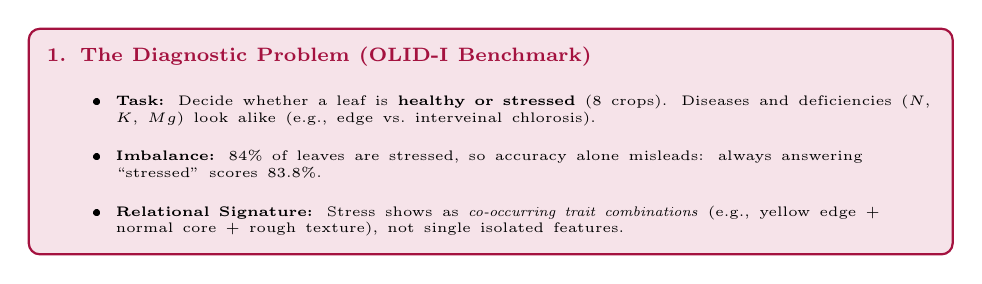
\begin{tikzpicture}
            \node[rectangle, draw=amritaMaroon, thick, fill=maroonSoft,
                  rounded corners=4pt, inner sep=6.5pt, text width=0.93\columnwidth, align=left] {
                {\scriptsize\bfseries\textcolor{amritaMaroon}{1. The Diagnostic Problem (OLID-I Benchmark)}}\\[3pt]
                \begin{itemize}\tiny
                    \item \textbf{Task:} Decide whether a leaf is \textbf{healthy or stressed} (8 crops). Diseases and deficiencies ($\text{N}$, $\text{K}$, $\text{Mg}$) look alike (e.g., edge vs.\ interveinal chlorosis).
                    \item \textbf{Imbalance:} 84\% of leaves are stressed, so accuracy alone misleads: always answering ``stressed'' scores 83.8\%.
                    \item \textbf{Relational Signature:} Stress shows as \emph{co-occurring trait combinations} (e.g., yellow edge + normal core + rough texture), not single isolated features.
                \end{itemize}
            };
        \end{tikzpicture}

        \vspace{0.15cm}
        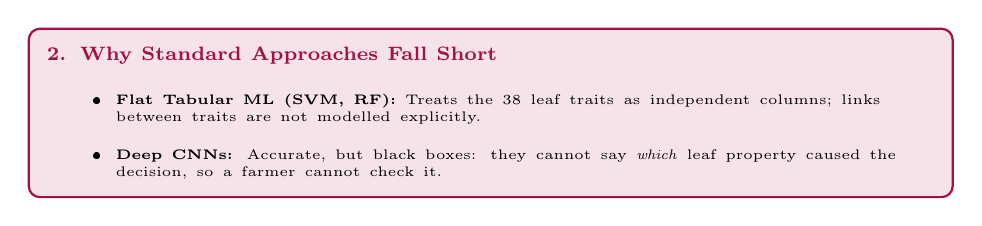
\begin{tikzpicture}
            \node[rectangle, draw=amritaMaroon, thick, fill=maroonSoft,
                  rounded corners=4pt, inner sep=6.5pt, text width=0.93\columnwidth, align=left] {
                {\scriptsize\bfseries\textcolor{amritaMaroon}{2. Why Standard Approaches Fall Short}}\\[3pt]
                \begin{itemize}\tiny
                    \item \textbf{Flat Tabular ML (SVM, RF):} Treats the 38 leaf traits as independent columns; links between traits are not modelled explicitly.
                    \item \textbf{Deep CNNs:} Accurate, but black boxes: they cannot say \emph{which} leaf property caused the decision, so a farmer cannot check it.
                \end{itemize}
            };
        \end{tikzpicture}

        % --- Right Column: Why WL Kernel + Research Gap ---
        \column{0.485\textwidth}
        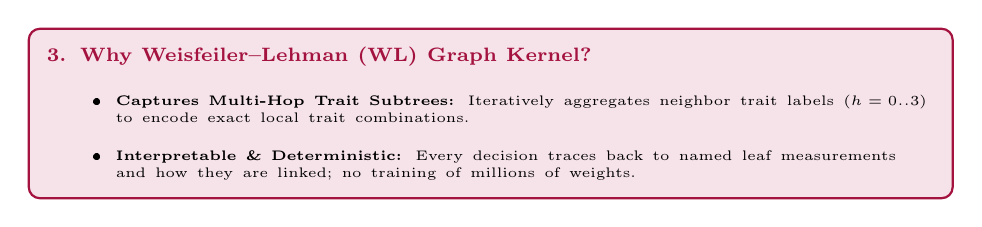
\begin{tikzpicture}
            \node[rectangle, draw=amritaMaroon, thick, fill=maroonSoft,
                  rounded corners=4pt, inner sep=6.5pt, text width=0.93\columnwidth, align=left] {
                {\scriptsize\bfseries\textcolor{amritaMaroon}{3. Why Weisfeiler--Lehman (WL) Graph Kernel?}}\\[3pt]
                \begin{itemize}\tiny
                    \item \textbf{Captures Multi-Hop Trait Subtrees:} Iteratively aggregates neighbor trait labels ($h=0..3$) to encode exact local trait combinations.
                    \item \textbf{Interpretable \& Deterministic:} Every decision traces back to named leaf measurements and how they are linked; no training of millions of weights.
                \end{itemize}
            };
        \end{tikzpicture}

        \vspace{0.15cm}
        
\begin{tikzpicture}
            \node[rectangle, draw=amritaMaroon, very thick, fill=amritaMaroon, text=white,
                  rounded corners=4pt, inner sep=7pt, text width=0.93\columnwidth, align=left] {
                {\tiny\bfseries\textcolor{maroonSoft}{THE UNSOLVED RESEARCH GAP}}\\[3pt]
                {\scriptsize A leaf image is \textbf{not naturally a graph}. Since WL performance depends entirely on graph edges, \emph{which graph topology best models leaf trait relationships?}}
            };
        \end{tikzpicture}
    \end{columns}
\end{frame}
% ============================================================
% FRAME: How Does WL Work? -- Visual Demonstration
% ============================================================
\begin{frame}{How Does WL Work?}

    \begin{center}
        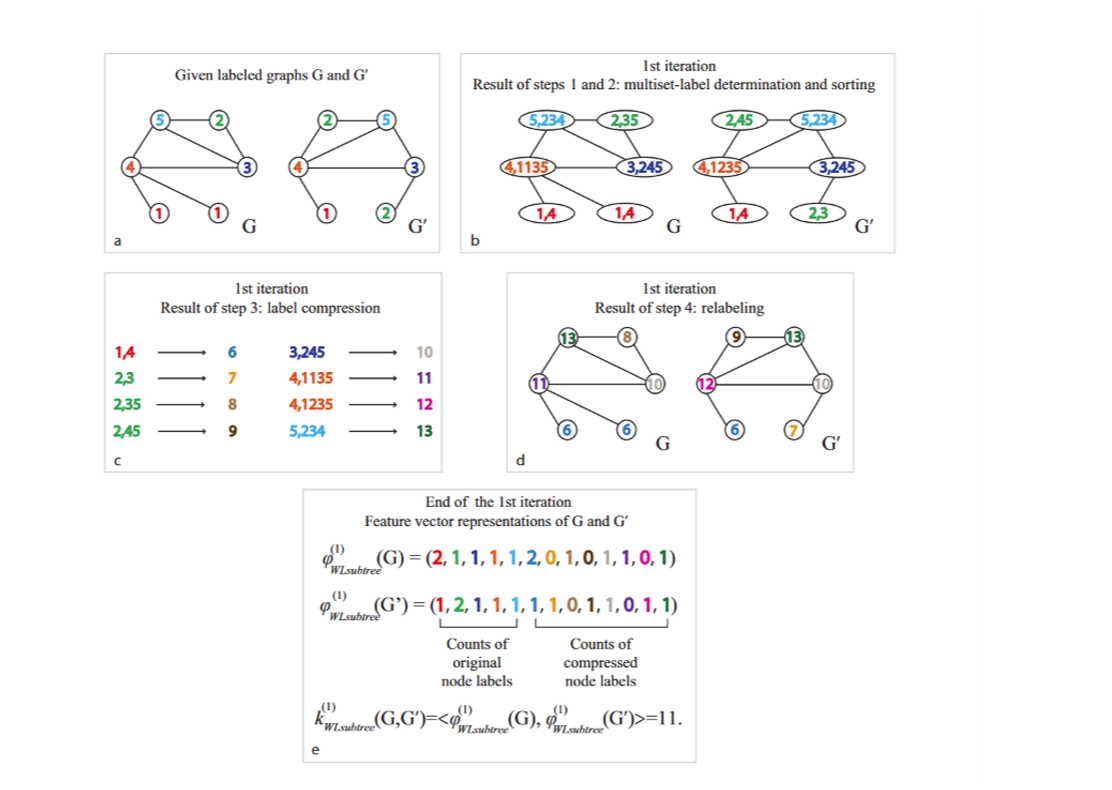
\includegraphics[width=0.85\textwidth, height=0.75\textheight, keepaspectratio]{image.png}
    \end{center}

    \vspace{-0.15cm}
    \begin{center}
        {\scriptsize\itshape Subtree neighborhood aggregation in the Weisfeiler--Lehman framework \cite{shervashidze2011weisfeiler}.}
    \end{center}

    \note{The main technique used in this research is the Weisfeiler--Lehman graph
    kernel \cite{shervashidze2011weisfeiler}. WL starts with the labels of the nodes and iteratively updates each
    node's label based on its own label and the labels of its neighbors.}
\end{frame}

% ============================================================
% SLIDE 4: WL Algorithm -- Mathematical Formulation
% ============================================================
\begin{frame}{WL Algorithm: Mathematical Formulation}
    \framesubtitle{Iterative multiset aggregation and injective label compression \cite{weisfeiler1968reduction, shervashidze2011weisfeiler}}

    % --- Highlighted Formula Banner ---
    \begin{center}
        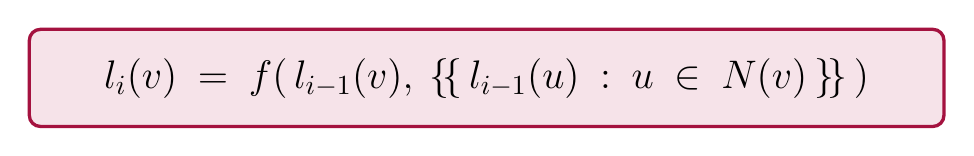
\begin{tikzpicture}
            \node[rectangle, draw=amritaMaroon, very thick, fill=maroonSoft,
                  rounded corners=4pt, inner sep=10pt, text width=0.90\textwidth, align=center] {
                {\Large $\displaystyle l_i(v) = f\Big(\, l_{i-1}(v),\ \{\!\{\, l_{i-1}(u) : u \in N(v) \,\}\!\}\,\Big)$}
            };
        \end{tikzpicture}
    \end{center}

    \vspace{0.2cm}

    % --- 4 Structured Explanation Cards (2x2 Grid) ---
    \begin{columns}[T, onlytextwidth]
        \column{0.485\textwidth}
        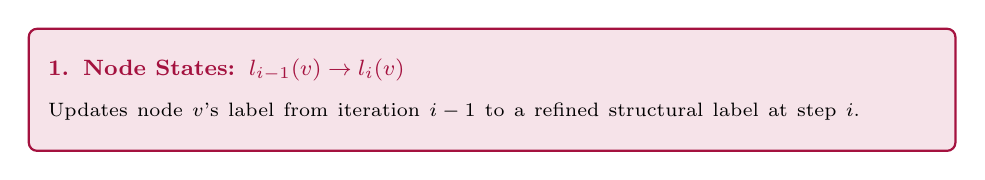
\begin{tikzpicture}
            \node[rectangle, draw=amritaMaroon, thick, fill=maroonSoft,
                  rounded corners=3pt, inner sep=7pt, text width=0.93\columnwidth, minimum height=1.55cm, align=left] {
                {\footnotesize\bfseries\textcolor{amritaMaroon}{1. Node States: $l_{i-1}(v) \rightarrow l_i(v)$}}\\[3pt]
                {\scriptsize Updates node $v$'s label from iteration $i-1$ to a refined structural label at step $i$.}
            };
        \end{tikzpicture}

        \vspace{0.18cm}
        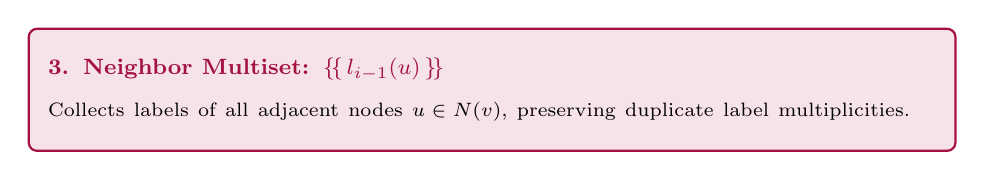
\begin{tikzpicture}
            \node[rectangle, draw=amritaMaroon, thick, fill=maroonSoft,
                  rounded corners=3pt, inner sep=7pt, text width=0.93\columnwidth, minimum height=1.55cm, align=left] {
                {\footnotesize\bfseries\textcolor{amritaMaroon}{3. Neighbor Multiset: $\{\!\{\, l_{i-1}(u) \,\}\!\}$}}\\[3pt]
                {\scriptsize Collects labels of all adjacent nodes $u \in N(v)$, preserving duplicate label multiplicities.}
            };
        \end{tikzpicture}

        \column{0.485\textwidth}
        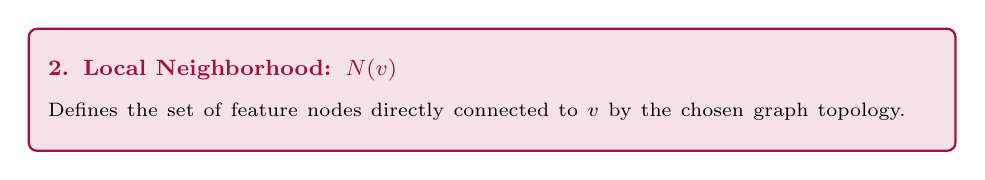
\begin{tikzpicture}
            \node[rectangle, draw=amritaMaroon, thick, fill=maroonSoft,
                  rounded corners=3pt, inner sep=7pt, text width=0.93\columnwidth, minimum height=1.55cm, align=left] {
                {\footnotesize\bfseries\textcolor{amritaMaroon}{2. Local Neighborhood: $N(v)$}}\\[3pt]
                {\scriptsize Defines the set of feature nodes directly connected to $v$ by the chosen graph topology.}
            };
        \end{tikzpicture}

        \vspace{0.18cm}
        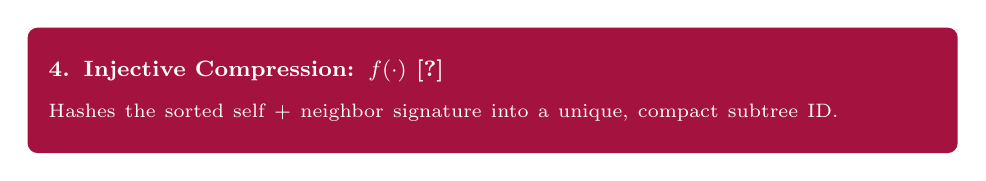
\begin{tikzpicture}
            \node[rectangle, draw=amritaMaroon, very thick, fill=amritaMaroon, text=white,
                  rounded corners=3pt, inner sep=7pt, text width=0.93\columnwidth, minimum height=1.55cm, align=left] {
                {\footnotesize\bfseries 4. Injective Compression: $f(\cdot)$ \cite{shervashidze2011weisfeiler}}\\[3pt]
                {\scriptsize Hashes the sorted self + neighbor signature into a unique, compact subtree ID.}
            };
        \end{tikzpicture}
    \end{columns}
\end{frame}


% ============================================================
% FRAME: Applications in the Literature (evidence slide)
% ============================================================
% \begin{frame}{Applications in the Literature}
%     \framesubtitle{WL graph kernels power real detection and comparison systems}

%     \begin{center}
%     \begin{tikzpicture}[every node/.style={transform shape}]
%         \node[anchor=north west, inner sep=4pt, fill=maroonSoft, draw=amritaMaroon, thick, rounded corners=3pt, minimum width=2.4cm, minimum height=1.35cm, align=center] (img1) at (0,0)
%             {\iconMagnify\\[1pt]\tiny\textbf{Behavior Graphs}};
%         \node[anchor=north west, text width=8.8cm, align=left] (txt1) at (2.8,0.05) {
%             \footnotesize\textbf{Malware Detection}\\[2pt]
%             \scriptsize A \emph{contextual} WL graph kernel over program
%             behavior graphs distinguishes malware from benign software
%             \cite{narayanan2016contextual}.
%         };

%         \node[anchor=north west, inner sep=4pt, fill=maroonSoft, draw=amritaMaroon, thick, rounded corners=3pt, minimum width=2.4cm, minimum height=1.35cm, align=center] (img2) at (0,-1.9)
%             {\iconGraph\\[1pt]\tiny\textbf{Program AST / CFG}};
%         \node[anchor=north west, text width=8.8cm, align=left] (txt2) at (2.8,-1.85) {
%             \footnotesize\textbf{Program Similarity Detection}\\[2pt]
%             \scriptsize The WL kernel compares program graphs directly to
%             detect similar or cloned code, without hand-crafted features
%             \cite{li2016detecting}.
%         };

%         \node[anchor=north west, inner sep=4pt, fill=maroonSoft, draw=amritaMaroon, thick, rounded corners=3pt, minimum width=2.4cm, minimum height=1.35cm, align=center] (img3) at (0,-3.8)
%             {\iconDNA\\[1pt]\tiny\textbf{Protein Topology}};
%         \node[anchor=north west, text width=8.8cm, align=left] (txt3) at (2.8,-3.75) {
%             \footnotesize\textbf{Bioinformatics -- Protein Function}\\[2pt]
%             \scriptsize Amino-acid-level protein graphs, scored with WL
%             kernels, support \textbf{protein function} and phenotype
%             prediction \cite{borgwardt2005protein, shervashidze2011weisfeiler} -- the same principle used here for plant traits.
%         };
%     \end{tikzpicture}
%     \end{center}

%     \vspace{0.05cm}
%     {\scriptsize\itshape Across security, software engineering, and biology,
%     the same idea recurs: represent structure as a graph, let WL capture
%     its neighborhoods, and compare.}
% \end{frame}
% ============================================================
% SLIDE 5: How Does the WL Graph Kernel Perform Classification?
% ============================================================
\begin{frame}{How Does the WL Graph Kernel Perform Classification?}
    \framesubtitle{End-to-end structural classification pipeline from feature graph to stress prediction}

    \vspace{0.05cm}
    \begin{center}
    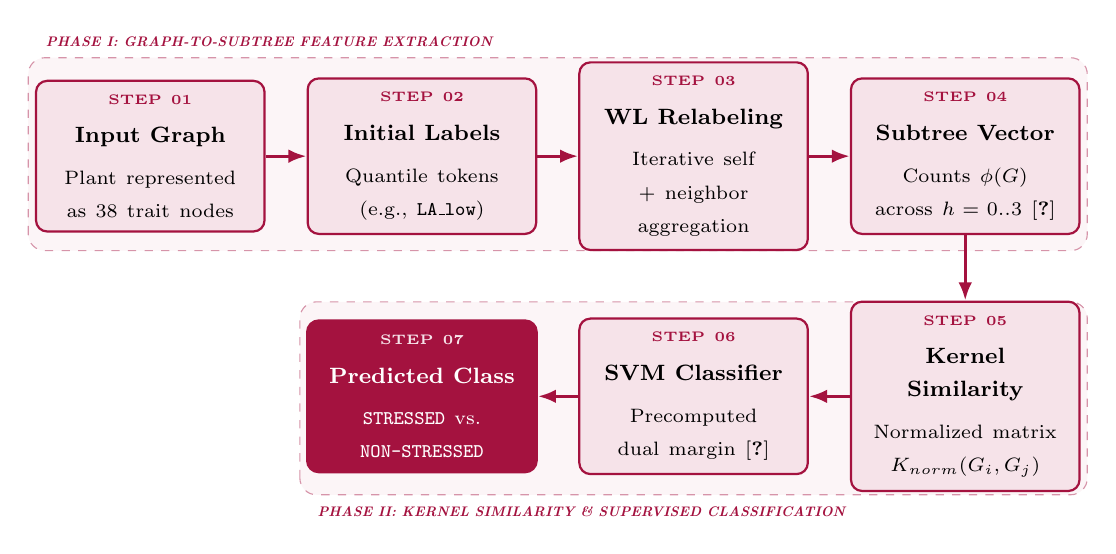
\begin{tikzpicture}[
        stagecard/.style={
            rectangle, draw=amritaMaroon, thick, fill=maroonSoft,
            rounded corners=4pt, text width=2.55cm, minimum height=1.75cm,
            inner sep=5pt, align=center
        },
        finalcard/.style={
            rectangle, draw=amritaMaroon, very thick, fill=amritaMaroon, text=white,
            rounded corners=4pt, text width=2.55cm, minimum height=1.75cm,
            inner sep=5pt, align=center
        }
    ]
        % --- Phase I Container & Top Header ---
        \draw[fill=maroonSoft!35, draw=amritaMaroon!45, dashed, rounded corners=6pt]
            (-1.55,-1.05) rectangle (11.90,1.40);
        \node[font=\tiny\bfseries\itshape, text=amritaMaroon, anchor=south west]
            at (-1.45, 1.42) {PHASE I: GRAPH-TO-SUBTREE FEATURE EXTRACTION};

        % --- Phase II Container & Bottom Header ---
        \draw[fill=maroonSoft!35, draw=amritaMaroon!45, dashed, rounded corners=6pt]
            (1.90,-4.15) rectangle (11.90,-1.70);
        \node[font=\tiny\bfseries\itshape, text=amritaMaroon, anchor=north west]
            at (2.00, -4.18) {PHASE II: KERNEL SIMILARITY \& SUPERVISED CLASSIFICATION};

        % --- Row 1: Left to Right (y = 0.15) ---
        \node[stagecard] (s1) at (0, 0.15) {
            {\tiny\bfseries\textcolor{amritaMaroon}{STEP 01}}\\[2pt]
            {\footnotesize\bfseries Input Graph}\\[3pt]
            {\scriptsize Plant represented as 38 trait nodes}
        };

        \node[stagecard] (s2) at (3.45, 0.15) {
            {\tiny\bfseries\textcolor{amritaMaroon}{STEP 02}}\\[2pt]
            {\footnotesize\bfseries Initial Labels}\\[3pt]
            {\scriptsize Quantile tokens (e.g., \texttt{LA\_low})}
        };

        \node[stagecard] (s3) at (6.90, 0.15) {
            {\tiny\bfseries\textcolor{amritaMaroon}{STEP 03}}\\[2pt]
            {\footnotesize\bfseries WL Relabeling}\\[3pt]
            {\scriptsize Iterative self + neighbor aggregation}
        };

        \node[stagecard] (s4) at (10.35, 0.15) {
            {\tiny\bfseries\textcolor{amritaMaroon}{STEP 04}}\\[2pt]
            {\footnotesize\bfseries Subtree Vector}\\[3pt]
            {\scriptsize Counts $\phi(G)$ across $h = 0..3$ \cite{shervashidze2011weisfeiler}}
        };

        % --- Row 2: Right to Left (y = -2.90, clean vertical gap) ---
        \node[stagecard] (s5) at (10.35, -2.90) {
            {\tiny\bfseries\textcolor{amritaMaroon}{STEP 05}}\\[2pt]
            {\footnotesize\bfseries Kernel Similarity}\\[3pt]
            {\scriptsize Normalized matrix $K_{\text{norm}}(G_i, G_j)$}
        };

        \node[stagecard] (s6) at (6.90, -2.90) {
            {\tiny\bfseries\textcolor{amritaMaroon}{STEP 06}}\\[2pt]
            {\footnotesize\bfseries SVM Classifier}\\[3pt]
            {\scriptsize Precomputed dual margin \cite{cortes1995support}}
        };

        \node[finalcard] (s7) at (3.45, -2.90) {
            {\tiny\bfseries\textcolor{maroonSoft}{STEP 07}}\\[2pt]
            {\footnotesize\bfseries Predicted Class}\\[3pt]
            {\scriptsize \texttt{STRESSED} vs.\ \texttt{NON-STRESSED}}
        };

        % --- Clean Arrows ---
        \draw[-{Latex[length=2.3mm]}, very thick, draw=amritaMaroon] (s1) -- (s2);
        \draw[-{Latex[length=2.3mm]}, very thick, draw=amritaMaroon] (s2) -- (s3);
        \draw[-{Latex[length=2.3mm]}, very thick, draw=amritaMaroon] (s3) -- (s4);
        \draw[-{Latex[length=2.3mm]}, very thick, draw=amritaMaroon] (s4) -- (s5);
        \draw[-{Latex[length=2.3mm]}, very thick, draw=amritaMaroon] (s5) -- (s6);
        \draw[-{Latex[length=2.3mm]}, very thick, draw=amritaMaroon] (s6) -- (s7);
    \end{tikzpicture}
    \end{center}
\end{frame}

% ============================================================
% SLIDE 6: Dataset & Leaf Segmentation
% ============================================================
\begin{frame}{Dataset \& Leaf Segmentation}
    \framesubtitle{OLID dataset overview and Excess Green (ExG) foreground isolation \cite{orka2023olid, woebbecke1995color}}

    \begin{columns}[c, onlytextwidth]
        % --- Left Column: Dataset & Segmentation Cards ---
        \column{0.50\textwidth}
        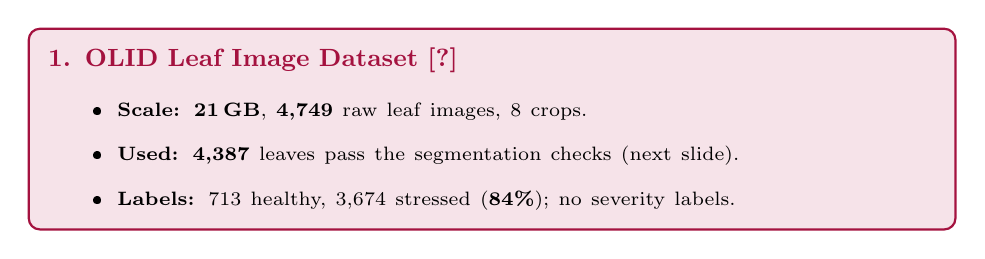
\begin{tikzpicture}
            \node[rectangle, draw=amritaMaroon, thick, fill=maroonSoft,
                  rounded corners=4pt, inner sep=7pt, text width=0.93\columnwidth, align=left] {
                {\small\bfseries\textcolor{amritaMaroon}{1. OLID Leaf Image Dataset \cite{orka2023olid}}}\\[4pt]
                \begin{itemize}\scriptsize
                    \item \textbf{Scale:} \textbf{21\,GB}, \textbf{4,749} raw leaf images, 8 crops.
                    \item \textbf{Used:} \textbf{4,387} leaves pass the segmentation checks (next slide).
                    \item \textbf{Labels:} 713 healthy, 3,674 stressed (\textbf{84\%}); no severity labels.
                \end{itemize}
            };
        \end{tikzpicture}

        \vspace{0.18cm}
        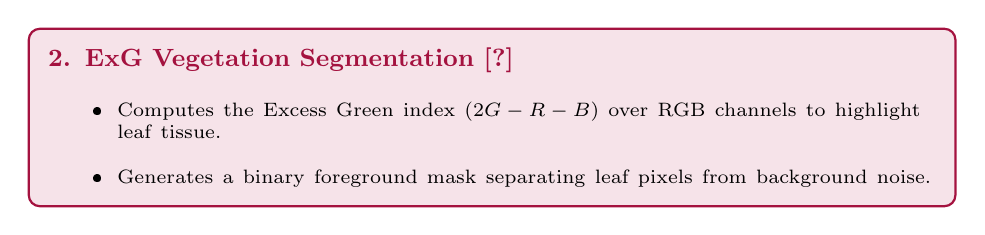
\begin{tikzpicture}
            \node[rectangle, draw=amritaMaroon, thick, fill=maroonSoft,
                  rounded corners=4pt, inner sep=7pt, text width=0.93\columnwidth, align=left] {
                {\small\bfseries\textcolor{amritaMaroon}{2. ExG Vegetation Segmentation \cite{woebbecke1995color}}}\\[4pt]
                \begin{itemize}\scriptsize
                    \item Computes the Excess Green index ($2G - R - B$) over RGB channels to highlight leaf tissue.
                    \item Generates a binary foreground mask separating leaf pixels from background noise.
                \end{itemize}
            };
        \end{tikzpicture}

        % --- Right Column: Combined Data Processing Visual ---
        \column{0.47\textwidth}
        \centering
        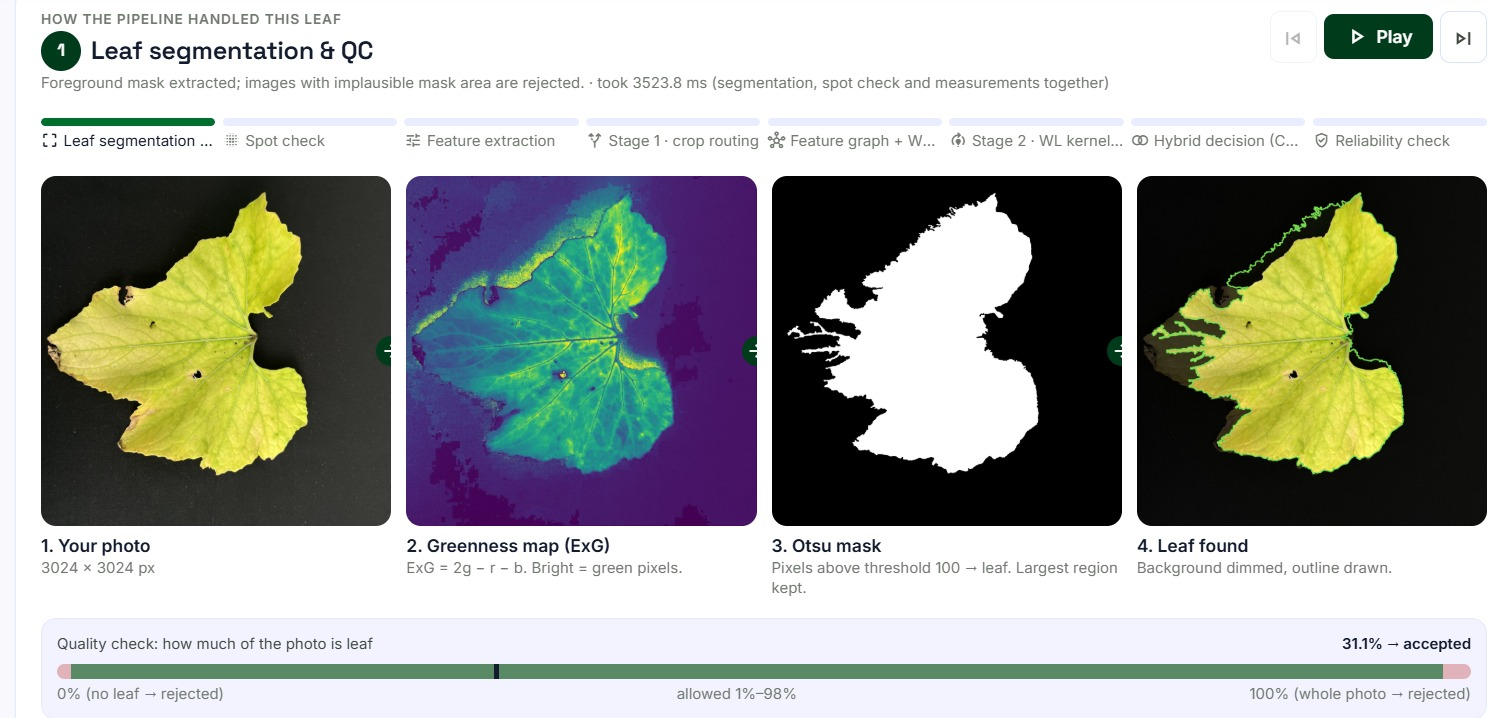
\includegraphics[width=0.95\linewidth, height=0.65\textheight, keepaspectratio]{dataprocess.jpg}\\[4pt]
        {\tiny\itshape Data processing and ExG leaf segmentation pipeline}
    \end{columns}
\end{frame}

% ============================================================
% SLIDE 7: Segmentation Validation: Rules & Visual Examples
% ============================================================
\begin{frame}{Segmentation Validation: Rules \& Visual Examples}
    \framesubtitle{Otsu-based mask area ratio filtering to discard distorted segmentations \cite{otsu1979threshold}}

    \begin{columns}[c, onlytextwidth]
        % --- Left Column: Formula & Acceptance Rules ---
        \column{0.49\textwidth}
        
\begin{tikzpicture}
            \node[rectangle, draw=amritaMaroon, thick, fill=maroonSoft,
                  rounded corners=4pt, inner sep=7pt, text width=0.93\columnwidth, align=center] {
                {\scriptsize\bfseries\textcolor{amritaMaroon}{Otsu Mask Area Ratio \cite{otsu1979threshold}}}\\[4pt]
                {\small $\text{Ratio} = \dfrac{\text{Leaf mask area}}{\text{Total image area}}$}
            };
        \end{tikzpicture}

        \vspace{0.22cm}
        \begin{table}
            \centering
            \scriptsize
            \setlength{\tabcolsep}{3.5pt}
            \renewcommand{\arraystretch}{1.25}
            \begin{tabular}{@{}llp{2.9cm}@{}}
                \toprule
                \textbf{Condition} & \textbf{Status} & \textbf{Meaning} \\
                \midrule
                $\text{Ratio} < 0.01$ & \textcolor{red}{\bfseries FAILED} & Under-segmented / tiny mask \\
                $0.01 \le \text{Ratio} \le 0.98$ & \textcolor{green!60!black}{\bfseries ACCEPT} & Reasonable leaf segmentation \\
                $\text{Ratio} > 0.98$ & \textcolor{red}{\bfseries FAILED} & Over-segmented / flooded mask \\
                \bottomrule
            \end{tabular}
        \end{table}

        % --- Right Column: 2x2 Visual Grid of Accepted & Declined Samples ---
        \column{0.48\textwidth}
        \centering
        {\scriptsize\textbf{\textcolor{green!60!black}{Accepted Samples}} ($0.01 \le \text{Ratio} \le 0.98$)}\\[3pt]
        \begin{columns}[T, onlytextwidth]
            \column{0.48\textwidth}
            \centering
            \fcolorbox{green!60!black}{white}{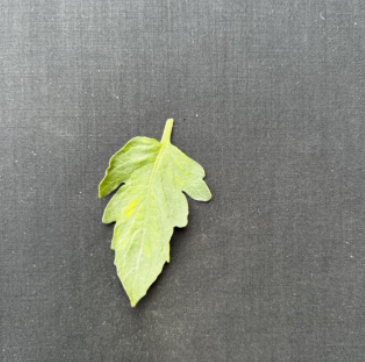
\includegraphics[width=2.0cm, height=1.3cm]{accepted_leaf1.png}}\\[2pt]
            {\tiny \textbf{Sample 1:} Ratio $\approx 0.0759$}

            \column{0.48\textwidth}
            \centering
            \fcolorbox{green!60!black}{white}{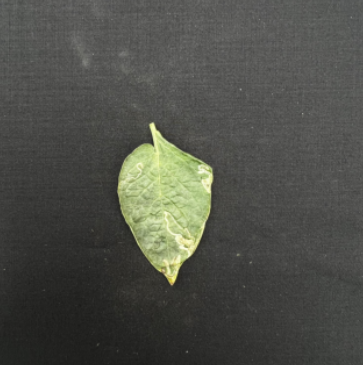
\includegraphics[width=2.0cm, height=1.3cm]{accepted_leaf2.png}}\\[2pt]
            {\tiny \textbf{Sample 2:} Ratio $\approx 0.1542$}
        \end{columns}

        \vspace{0.2cm}
        {\scriptsize\textbf{\textcolor{red}{Declined Samples}} ($\text{Ratio} < 0.01$ or $> 0.98$)}\\[3pt]
        \begin{columns}[T, onlytextwidth]
            \column{0.48\textwidth}
            \centering
            \fcolorbox{red}{white}{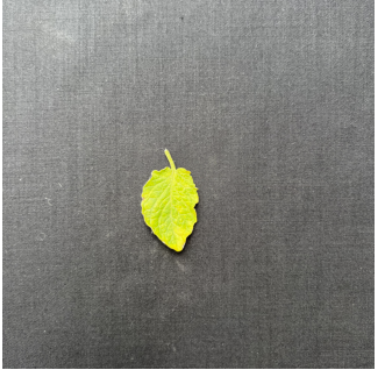
\includegraphics[width=2.0cm, height=1.3cm]{declined_empty.png}}\\[2pt]
            {\tiny \textbf{Over-segmented:} Ratio $= 0.99$}

            \column{0.48\textwidth}
            \centering
            \fcolorbox{red}{white}{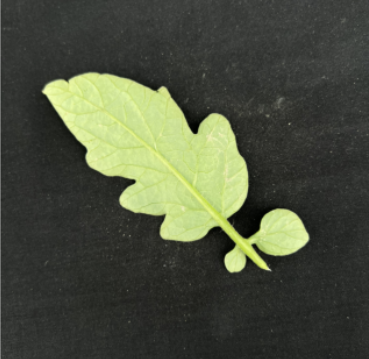
\includegraphics[width=2.0cm, height=1.3cm]{declined_flooded.png}}\\[2pt]
            {\tiny \textbf{Under-segmented:} Ratio $= 0.0002$}
        \end{columns}
    \end{columns}
\end{frame}

% % ============================================================
% % FRAME: Segmentation & Feature Sanity Checks
% % ============================================================
% \begin{frame}{Segmentation \& Feature  Checks}
%     \framesubtitle{Validating the dataset before graph construction}

%     \begin{columns}[c]
        
%         % Left: Acceptance
%         \column{0.50\textwidth}
%         \centering
%         \textbf{Segmentation Acceptance by Crop}\\[6pt]
%         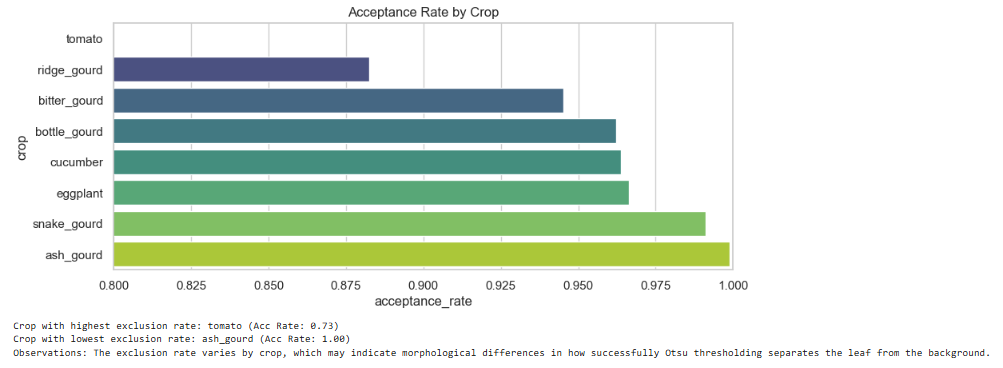
\includegraphics[width=0.95\linewidth]{haha.png}\\[5pt]
%         {\scriptsize
%         Acceptance varies across crops, with tomato showing the
%         highest exclusion and ash\_gourd the highest acceptance.
%         }

%         % Right: Sanity checks
%         \column{0.48\textwidth}
%         \centering
%         \textbf{Feature Checks}\\[0.4cm]

%         \renewcommand{\arraystretch}{1.2}
%         \begin{tabular}{@{}c@{\hspace{10pt}}l@{}}
%             \iconCheck & \textbf{NaN / Infinite Values} \\[12pt]
%             \iconCheck & \textbf{Constant Features}     \\[12pt]
%             \iconCheck & \textbf{Duplicate Records}     \\[12pt]
%             \iconCheck & \textbf{Outliers}
%         \end{tabular}

%     \end{columns}

% \end{frame}


% % ============================================================
% % FRAME: Feature Distributions
% % ============================================================
% \begin{frame}{Feature Distributions}
%     \framesubtitle{Visual inspection of the 38 extracted features}

%     \vspace{-0.25cm}
%     \begin{center}
%         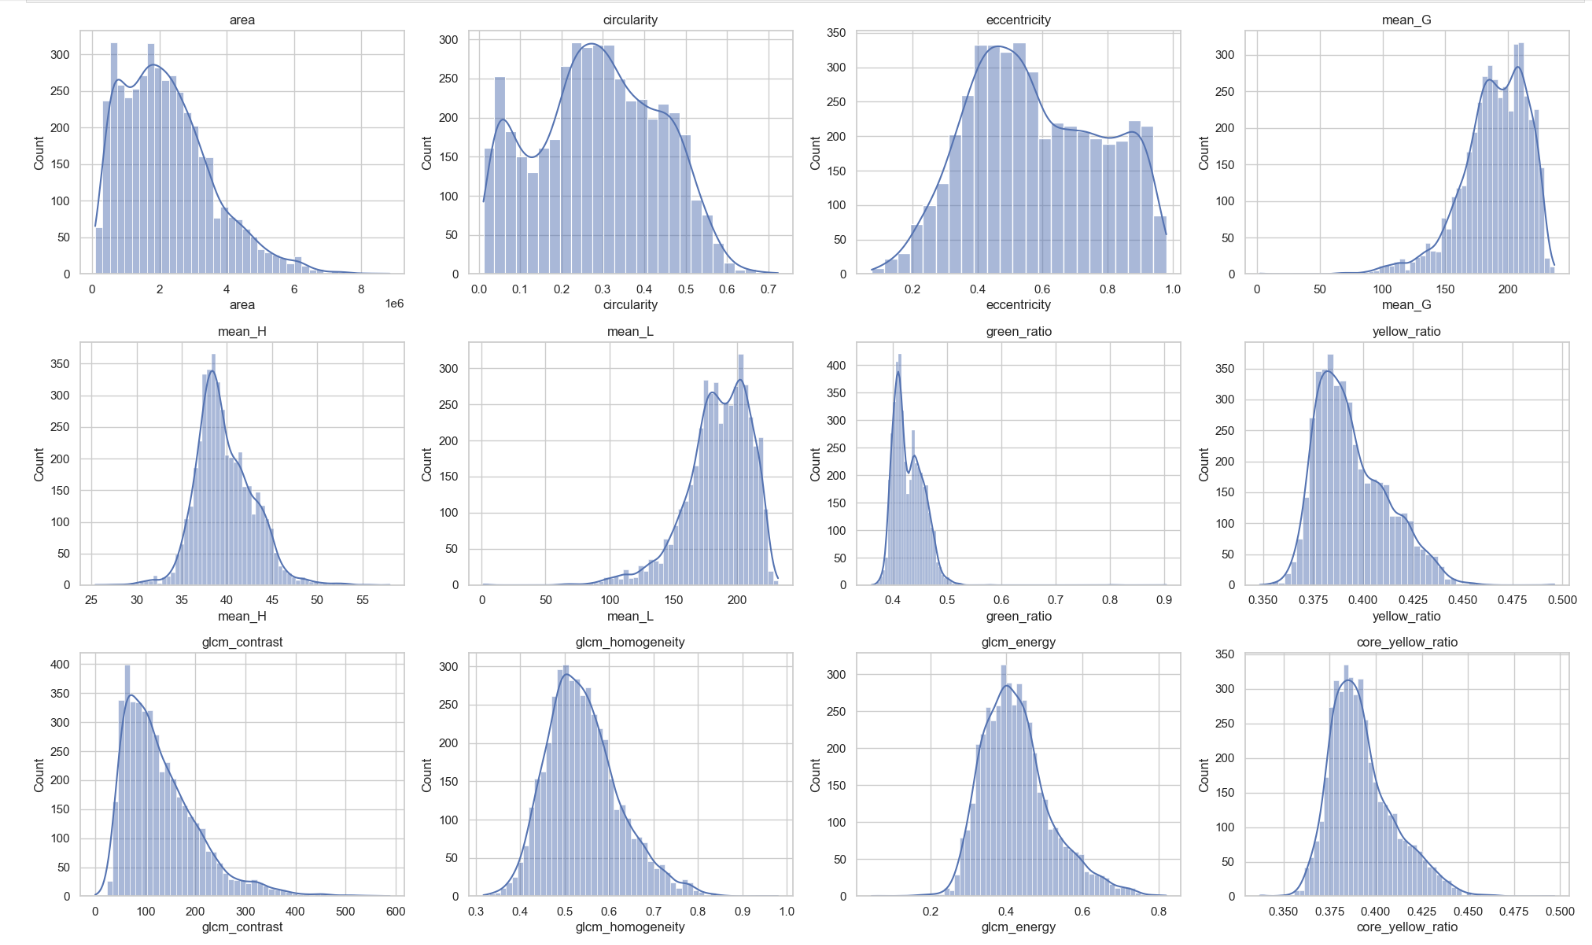
\includegraphics[width=0.88\textwidth, height=0.60\textheight, keepaspectratio]{feature_distributions.png}
%     \end{center}

%     \vspace{-0.15cm}
%     \begin{center}
%         {\scriptsize\itshape Histograms of shape, color, and texture features across the accepted dataset -- confirming reasonable spread and absence of degenerate distributions.}
%     \end{center}
% \end{frame}
% % ============================================================
% % FRAME: Mask Area Distribution of Entire Dataset
% % ============================================================
% \begin{frame}{Mask Area Distribution of Entire Dataset}
%     \framesubtitle{Population-level overview of segmentation area ratios}

%     \begin{center}
%         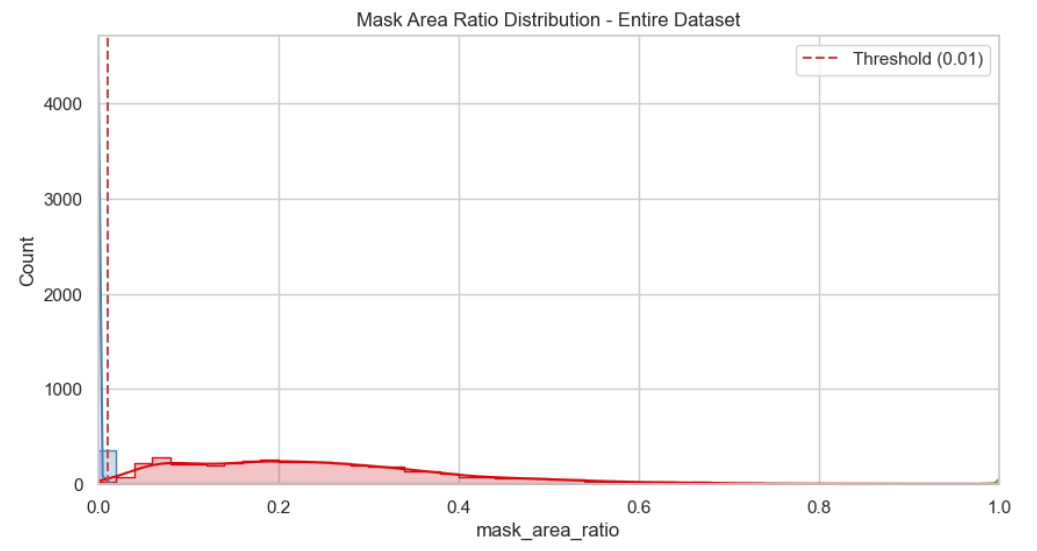
\includegraphics[width=0.78\textwidth, height=0.62\textheight, keepaspectratio]{wowow.png}
%     \end{center}

%     \vspace{-0.1cm}
%     {\scriptsize\itshape Distribution across all samples illustrating leaf-to-image coverage ratios prior to downstream feature extraction and graph mapping.}
% \end{frame}



% % ============================================================
% % FRAME: Dataset Filtering Summary
% % ============================================================
% \begin{frame}{Dataset Filtering Summary}
%     \framesubtitle{Overall throughput after Otsu-based mask area validation}

%     \begin{columns}[c]
%         \column{0.52\textwidth}
%         \begin{table}[]
%             \centering
%             \small
%             \begin{tabular}{lr}
%                 \toprule
%                 \textbf{Metric} & \textbf{Value} \\
%                 \midrule
%                 Original Samples & 4,749 \\
%                 Accepted Samples & \textbf{\textcolor{green!60!black}{4,387}} \\
%                 Excluded Samples & \textbf{\textcolor{red}{362}} \\
%                 \midrule
%                 \textbf{Overall Acceptance Rate} & \textbf{92.38\%} \\
%                 \bottomrule
%             \end{tabular}
%         \end{table}

%         \column{0.44\textwidth}
%         \begin{tikzpicture}
%             \node[rectangle, draw=amritaMaroon, thick, fill=maroonSoft, 
%                   rounded corners=3pt, inner sep=10pt, text width=0.88\textwidth] {
%                 \textbf{Key Takeaway}
%                 \vspace{0.2cm}\\
%                 \footnotesize
%                 \begin{itemize}\footnotesize
%                     \item Over \textbf{92\%} of leaf segmentations successfully met the morphological coverage criteria.
%                     \item \textbf{Tomato} exhibited the highest exclusion rate among all evaluated crops.
%                 \end{itemize}
%             };
%         \end{tikzpicture}
%     \end{columns}

%     \vspace{0.4cm}
%     \begin{center}
%         {\scriptsize\itshape High retention confirms the viability of automated thresholding while pruning failure modes before graph construction.}
%     \end{center}
% \end{frame}


% ============================================================
% SLIDE: Feature Extraction (38 Traits) & Node Discretization
% ============================================================
\begin{frame}{Feature Extraction \& Graph Node Discretization}
    \framesubtitle{38 morphological, color, texture, and spatial traits quantized into discrete node labels \cite{haralick1973textural, pedregosa2011scikit}}

    \begin{columns}[T, onlytextwidth]
        % --- Left Column: 38 Extracted Features (4 Domain Cards) ---
        \column{0.58\textwidth}
        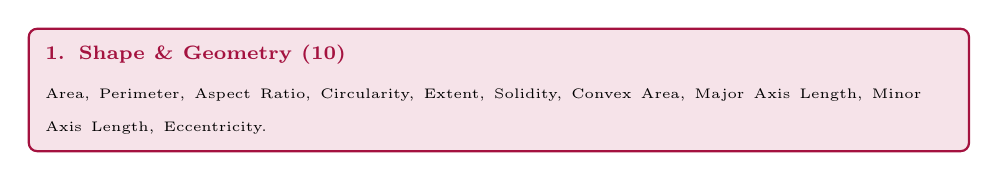
\begin{tikzpicture}
            \node[rectangle, draw=amritaMaroon, thick, fill=maroonSoft,
                  rounded corners=3pt, inner sep=6pt, text width=0.95\columnwidth, align=left] {
                {\scriptsize\bfseries\textcolor{amritaMaroon}{1. Shape \& Geometry (10)}}\\[2pt]
                {\tiny Area, Perimeter, Aspect Ratio, Circularity, Extent, Solidity, Convex Area, Major Axis Length, Minor Axis Length, Eccentricity.}
            };
        \end{tikzpicture}

        \vspace{0.12cm}
        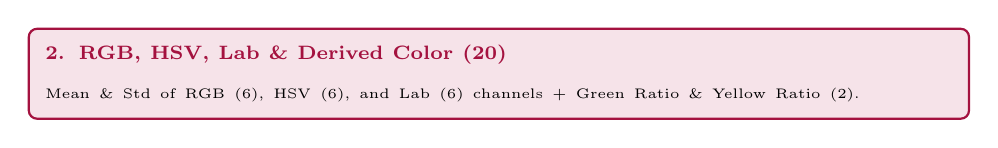
\begin{tikzpicture}
            \node[rectangle, draw=amritaMaroon, thick, fill=maroonSoft,
                  rounded corners=3pt, inner sep=6pt, text width=0.95\columnwidth, align=left] {
                {\scriptsize\bfseries\textcolor{amritaMaroon}{2. RGB, HSV, Lab \& Derived Color (20)}}\\[2pt]
                {\tiny Mean \& Std of RGB (6), HSV (6), and Lab (6) channels + Green Ratio \& Yellow Ratio (2).}
            };
        \end{tikzpicture}

        \vspace{0.12cm}
        \begin{columns}[T, onlytextwidth]
            \column{0.485\textwidth}
            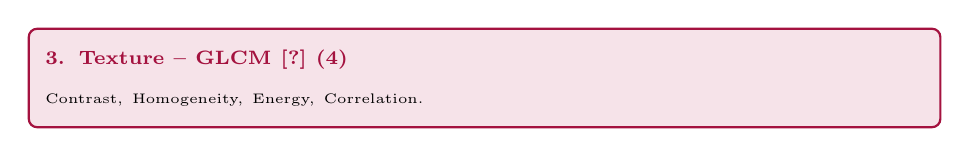
\begin{tikzpicture}
                \node[rectangle, draw=amritaMaroon, thick, fill=maroonSoft,
                      rounded corners=3pt, inner sep=6pt, text width=0.92\columnwidth, minimum height=1.25cm, align=left] {
                    {\scriptsize\bfseries\textcolor{amritaMaroon}{3. Texture -- GLCM \cite{haralick1973textural} (4)}}\\[2pt]
                    {\tiny Contrast, Homogeneity, Energy, Correlation.}
                };
            \end{tikzpicture}

            \column{0.485\textwidth}
            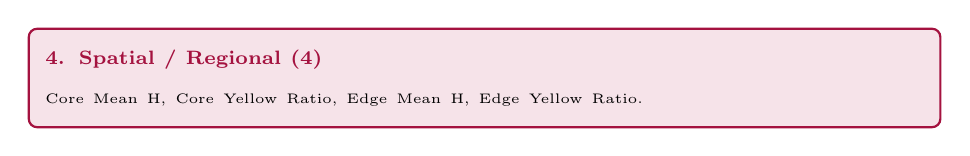
\begin{tikzpicture}
                \node[rectangle, draw=amritaMaroon, thick, fill=maroonSoft,
                      rounded corners=3pt, inner sep=6pt, text width=0.92\columnwidth, minimum height=1.25cm, align=left] {
                    {\scriptsize\bfseries\textcolor{amritaMaroon}{4. Spatial / Regional (4)}}\\[2pt]
                    {\tiny Core Mean H, Core Yellow Ratio, Edge Mean H, Edge Yellow Ratio.}
                };
            \end{tikzpicture}
        \end{columns}

        % --- Right Column: Quantile Discretization into Node Labels ---
        \column{0.39\textwidth}
        
\begin{tikzpicture}
            \node[rectangle, draw=amritaMaroon, very thick, fill=amritaMaroon, text=white,
                  rounded corners=4pt, inner sep=7pt, text width=0.93\columnwidth, align=left] {
                {\scriptsize\bfseries Quantile Node Labeling ($k = 3$)}\\[3pt]
                {\tiny Each of the \textbf{38 features} becomes a node, binned by quantile \cite{pedregosa2011scikit, dougherty1995supervised}. Labels keep the feature name (\texttt{area::High} $\neq$ \texttt{green\_ratio::High}); bins come from training folds only.}
            };
        \end{tikzpicture}

        \vspace{0.06cm}
        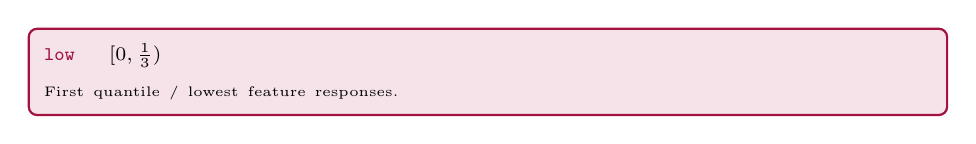
\begin{tikzpicture}
            \node[rectangle, draw=amritaMaroon, thick, fill=maroonSoft,
                  rounded corners=3pt, inner sep=5.5pt, text width=0.93\columnwidth, align=left] {
                {\scriptsize\bfseries\textcolor{amritaMaroon}{\texttt{low}} \quad $[0, \frac{1}{3})$}\\[1pt]
                {\tiny First quantile / lowest feature responses.}
            };
        \end{tikzpicture}

        \vspace{0.05cm}
        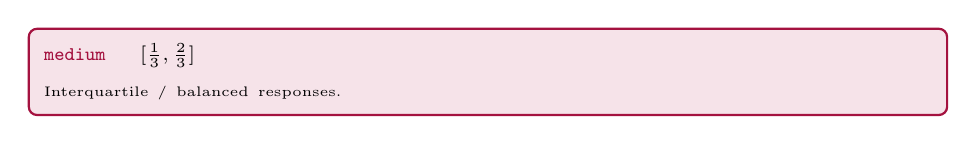
\begin{tikzpicture}
            \node[rectangle, draw=amritaMaroon, thick, fill=maroonSoft,
                  rounded corners=3pt, inner sep=5.5pt, text width=0.93\columnwidth, align=left] {
                {\scriptsize\bfseries\textcolor{amritaMaroon}{\texttt{medium}} \quad $[\frac{1}{3}, \frac{2}{3}]$}\\[1pt]
                {\tiny Interquartile / balanced responses.}
            };
        \end{tikzpicture}

        \vspace{0.05cm}
        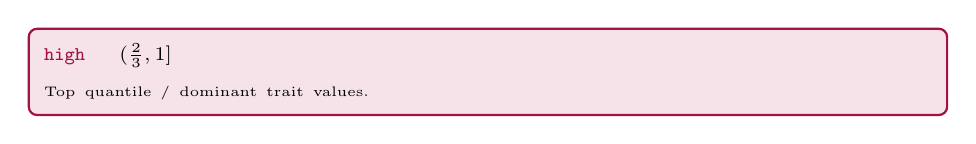
\begin{tikzpicture}
            \node[rectangle, draw=amritaMaroon, thick, fill=maroonSoft,
                  rounded corners=3pt, inner sep=5.5pt, text width=0.93\columnwidth, align=left] {
                {\scriptsize\bfseries\textcolor{amritaMaroon}{\texttt{high}} \quad $(\frac{2}{3}, 1]$}\\[1pt]
                {\tiny Top quantile / dominant trait values.}
            };
        \end{tikzpicture}
    \end{columns}
\end{frame}




% ============================================================
% SLIDE: Feature Application
% ============================================================
\begin{frame}{Example: One Leaf's 38 Measurements}
    \framesubtitle{A tomato leaf compared with the average healthy tomato leaf (from our PlantCare AI app)}

    \centering
    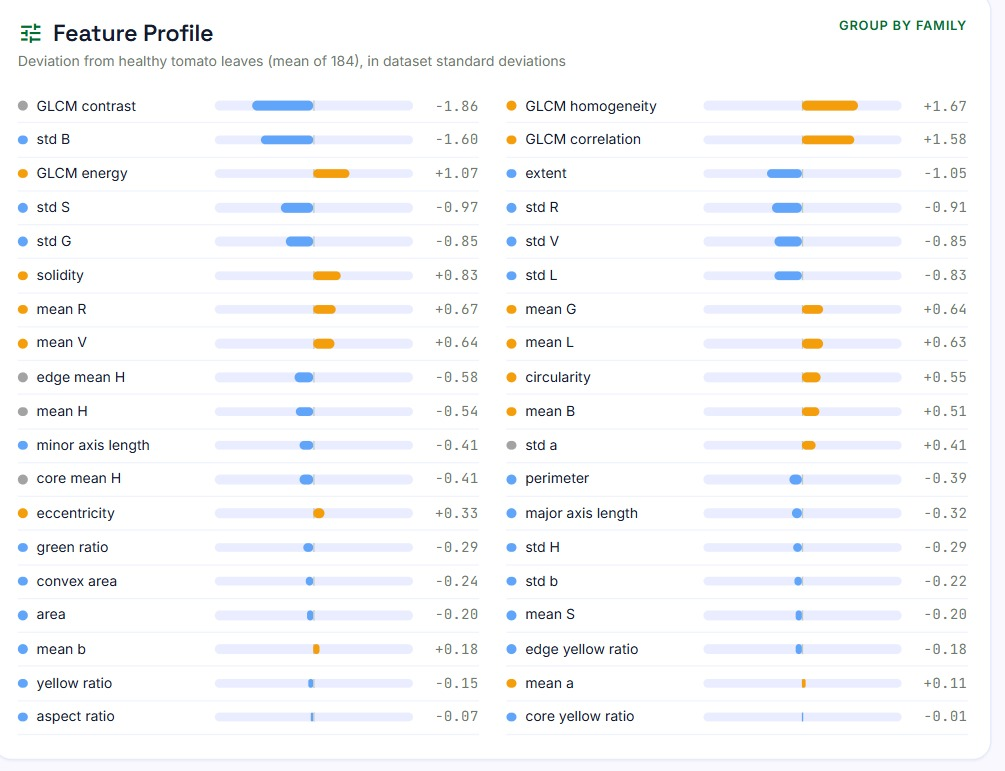
\includegraphics[width=0.92\textwidth, height=0.75\textheight, keepaspectratio]{feature_application.jpeg}\\[4pt]
    {\tiny\itshape Bars: how many standard deviations each measurement is from healthy tomato leaves. These differences are what the graph nodes encode.}
\end{frame}


% % ============================================================
% % FRAME: Continuous Feature Discretization
% % ============================================================
% \begin{frame}{Feature Discretization for Graph Labeling}
%     \framesubtitle{Converting continuous morphological traits into discrete node labels}

%     \textbf{Quantile-Based Discretization}
%     \vspace{0.15cm}

%     {\footnotesize To enable symbolic neighborhood aggregation in the \textbf{WL Graph Kernel}, continuous feature values are partitioned using \texttt{KBinsDiscretizer} (\texttt{strategy='quantile'}, $k=3$) \cite{pedregosa2011scikit, dougherty1995supervised}:}

%     \vspace{0.3cm}
%     \begin{itemize}\footnotesize
%         \item \textbf{\texttt{low} ($[0, \frac{1}{3})$):} First quantile / lowest feature responses.
%         \item \textbf{\texttt{medium} ($[\frac{1}{3}, \frac{2}{3}]$):} Interquartile / balanced feature responses.
%         \item \textbf{\texttt{high} ($(\frac{2}{3}, 1]$):} Top quantile / dominant feature values.
%     \end{itemize}

%     \vspace{0.45cm}
%     % \begin{tikzpicture}
%     %     \node[rectangle, draw=amritaMaroon, very thick, fill=maroonSoft,
%     %           rounded corners=3pt, inner sep=8pt, text width=0.92\textwidth] {
%     %         \footnotesize
%     %         \textbf{Impact on WL Initialization:} Continuous measurements (e.g., leaf area $\rightarrow 42.5\,\text{cm}^2$) are converted into discrete, categorical tokens (e.g., \texttt{LA\_low}, \texttt{LC\_high}) to initialize node labels prior to iterative neighborhood relabeling.
%     %     };
%     % \end{tikzpicture}
% \end{frame}
% ============================================================
% FRAME: Evaluated Graph Topologies (Clean Borderless Grid)
% ============================================================
\begin{frame}{Evaluated Graph Topologies (38 Feature Nodes)}
    \framesubtitle{Comparing five distinct edge-construction strategies for the WL kernel}

    % --- Top Row: 3 Graphs ---
    \begin{columns}[T, onlytextwidth]
        \column{0.32\textwidth}
        \centering
        {\scriptsize\bfseries\color{amritaMaroon} 1. Correlation Graph}\\[4pt]
        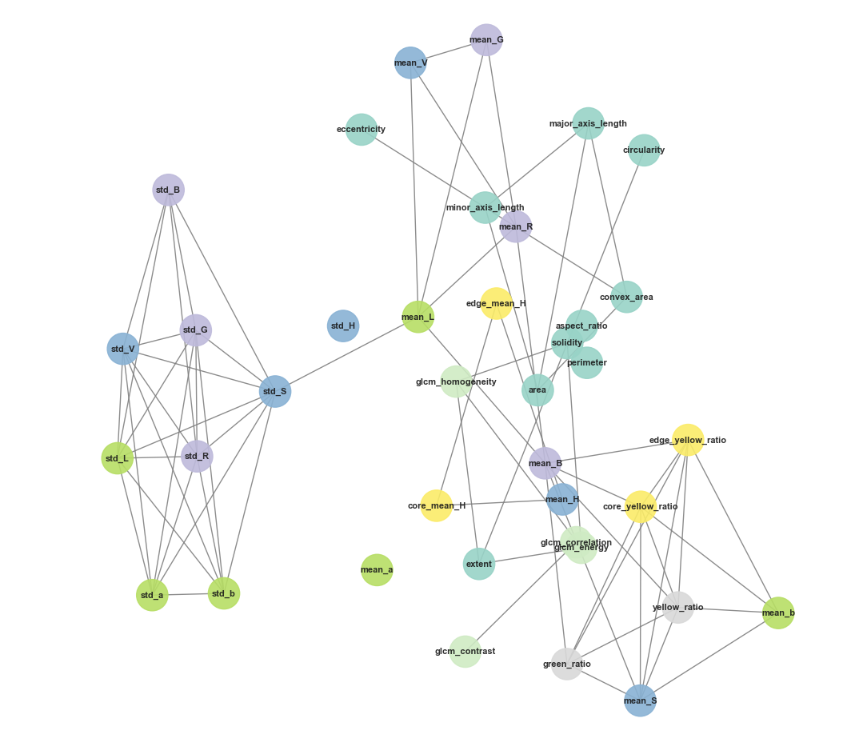
\includegraphics[width=\linewidth, height=0.25\textheight, keepaspectratio]{correlation_graph.png}\\[4pt]
        {\tiny Edge if $|r| \ge 0.70$ \cite{pearson1895notes}}

        \column{0.32\textwidth}
        \centering
        {\scriptsize\bfseries\color{amritaMaroon} 2. Feature-Similarity $K$-NN}\\[4pt]
        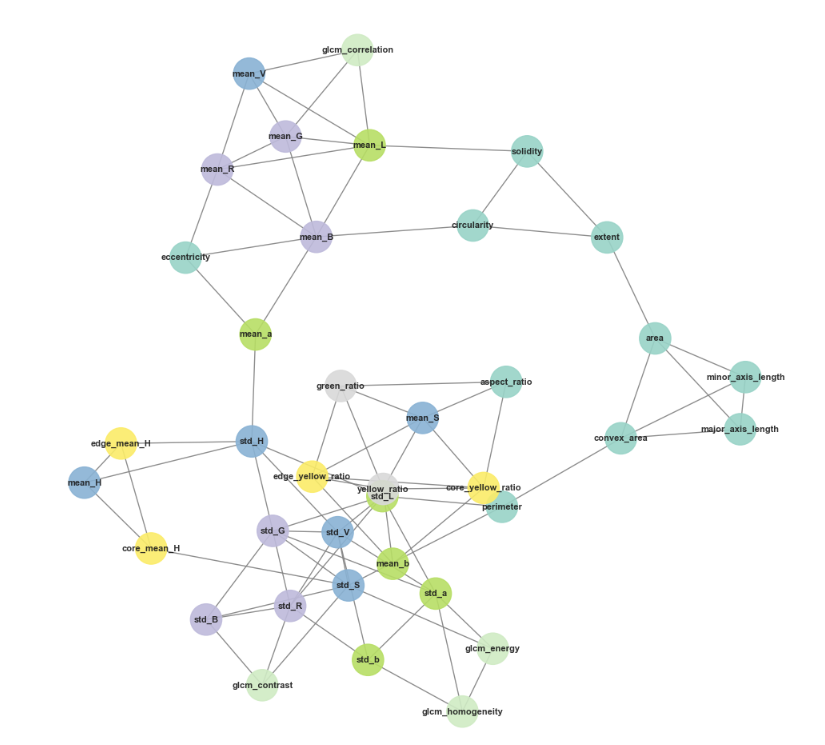
\includegraphics[width=\linewidth, height=0.25\textheight, keepaspectratio]{knn_Graph.png}\\[4pt]
        {\tiny Each trait linked to its $K{=}3$ closest traits \cite{cover1967nearest}}

        \column{0.32\textwidth}
        \centering
        {\scriptsize\bfseries\color{amritaMaroon} 3. Feature Family Graph}\\[4pt]
        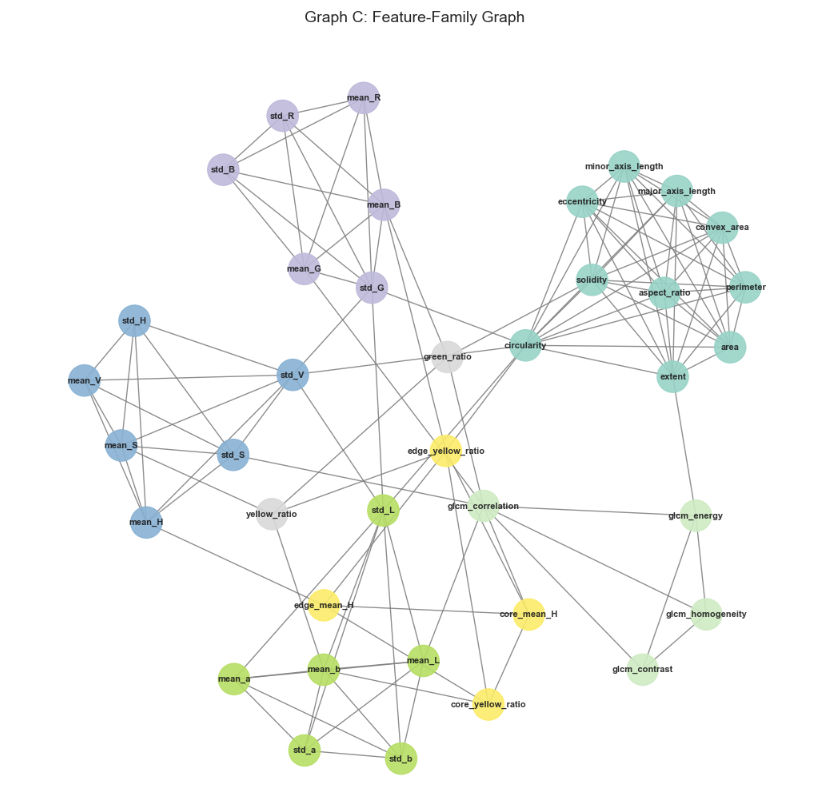
\includegraphics[width=\linewidth, height=0.25\textheight, keepaspectratio]{feature_family.png}\\[4pt]
        {\tiny 4 domain cliques + inter-family bridges}
    \end{columns}

    \vspace{0.3cm}

    % --- Bottom Row: 2 Centered Graphs ---
    \begin{columns}[T, onlytextwidth]
        \column{0.14\textwidth} % Left spacer

        \column{0.34\textwidth}
        \centering
        {\scriptsize\bfseries\color{amritaMaroon} 4. Spatial / Regional Graph}\\[4pt]
        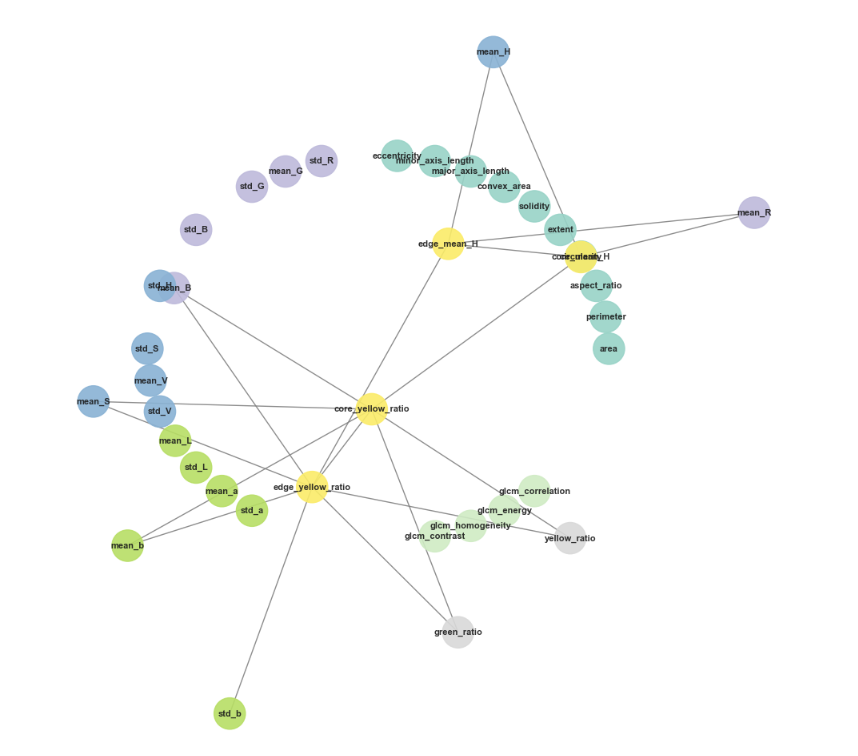
\includegraphics[width=\linewidth, height=0.25\textheight, keepaspectratio]{spatial_graph.png}\\[4pt]
        {\tiny Core--edge links + global traits ($|r| \ge 0.60$)}

        \column{0.34\textwidth}
        \centering
        {\scriptsize\bfseries\color{amritaMaroon} 5. Hybrid Graph}\\[4pt]
        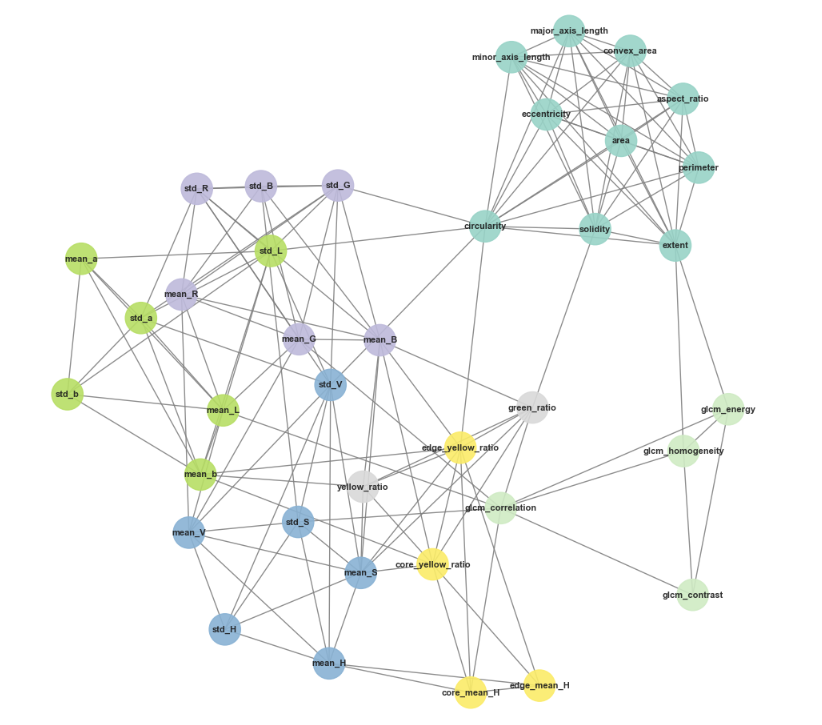
\includegraphics[width=\linewidth, height=0.25\textheight, keepaspectratio]{hybrid_graph.png}\\[4pt]
        {\tiny Union of Corr ($|r| \ge 0.8$), Family \& Spatial ($|r| \ge 0.7$)}

        \column{0.14\textwidth} % Right spacer
    \end{columns}
\end{frame}
% ============================================================
% FRAME: WL Iterations & Subtree Feature Vector (1/2)
% ============================================================
\begin{frame}{WL Iterations and the Subtree Feature Vector}
    \framesubtitle{Iterative label refinement from local features to larger subtrees \cite{shervashidze2011weisfeiler}}

    \begin{columns}[T]
        \column{0.48\textwidth}
        \textbf{1. Initial Node Labelling ($h = 0$)}
        \vspace{0.15cm}
        \begin{itemize}\footnotesize
            \item Each leaf is structured as a graph with \textbf{38 feature nodes}.
            \item Continuous feature values are mapped to categorical bins: \textbf{Low}, \textbf{Medium}, or \textbf{High}.
            % \item These form the baseline node labels ($h = 0$).
        \end{itemize}

        \vspace{0.3cm}
        \textbf{2. First Iteration ($h = 1$)}
        \vspace{0.15cm}
        \begin{itemize}\footnotesize
            \item For each node, WL aggregates:
            \begin{center}
                \scriptsize\texttt{Current Label} $+$ \texttt{Multiset of Neighbor Labels}
            \end{center}
            \item The combined string forms a \textbf{neighborhood signature}.
            \item Signatures are compressed into new, unique WL labels, capturing 1-hop local topology.
        \end{itemize}

        \column{0.48\textwidth}
        \textbf{3. Higher-Order Iterations ($h = 2, 3$)}
        \vspace{0.15cm}
        \begin{itemize}\footnotesize
            \item Output labels from iteration $h-1$ serve directly as input for iteration $h$.
            \item The multiset aggregation is repeated sequentially for depths \textbf{$h = 2$} and \textbf{$h = 3$}.
            \item With each hop, the compressed label captures an expanding subtree receptive field around each feature node.
        \end{itemize}

        \vspace{0.12cm}
        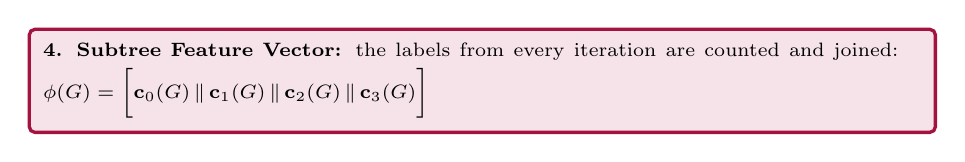
\begin{tikzpicture}
            \node[rectangle, draw=amritaMaroon, very thick, fill=maroonSoft,
                  rounded corners=2pt, inner sep=5pt, text width=0.92\columnwidth] {
                \scriptsize\textbf{4. Subtree Feature Vector:} the labels from every iteration are counted and joined:\\[2pt]
                \centering $\phi(G) = \big[\mathbf{c}_0(G) \,\|\, \mathbf{c}_1(G) \,\|\, \mathbf{c}_2(G) \,\|\, \mathbf{c}_3(G)\big]$
            };
        \end{tikzpicture}
    \end{columns}
\end{frame}

% ============================================================
% FRAME: WL Iterations & Subtree Feature Vector (2/2)
% ============================================================
% (merged into "WL Iterations and the Subtree Feature Vector")

% ============================================================
% FRAME: WL Subtree Feature Representations & Kernel Construction
% ============================================================
\begin{frame}{From Subtree Vectors to a Normalized Kernel}
    \framesubtitle{Pairwise leaf-graph similarity, computed inside each cross-validation fold \cite{shervashidze2011weisfeiler, scholkopf2002learning}}

    \begin{columns}[T]
        \column{0.48\textwidth}
        \textbf{1. Kernel Matrices (inner products)}
        \vspace{0.1cm}
        \begin{itemize}\footnotesize
            \item Stack the vectors $\phi(G)$ of all leaves into $\Phi$.
            \item \textbf{Training:} $K_{\text{train}} = \Phi_{\text{train}} \Phi_{\text{train}}^T$ \quad ($N_{\text{train}} \times N_{\text{train}}$)
            \item \textbf{Test fold:} $K_{\text{test}} = \Phi_{\text{test}} \Phi_{\text{train}}^T$ \quad ($N_{\text{test}} \times N_{\text{train}}$)
            \item Each entry counts the subtree patterns two leaves share.
        \end{itemize}

        \column{0.48\textwidth}
        \textbf{2. Cosine Normalization \cite{scholkopf2002learning}}
        \vspace{-0.1cm}
        \begin{equation*}
            K_{\text{norm}}(i,j) = \frac{K(i,j)}{\sqrt{K(i,i) \cdot K(j,j)}}
        \end{equation*}
        \vspace{-0.2cm}
        \begin{itemize}\footnotesize
            \item Similarity between 0 and 1; a leaf compared with itself gives 1.
            \item Removes the effect of how many labels a graph has, so only the \emph{pattern} counts.
        \end{itemize}
    \end{columns}

    \vspace{0.3cm}
    \begin{center}
        
\begin{tikzpicture}[node distance=0.4cm, auto, >=Latex]
            \tikzset{flowstep/.style={draw=amritaMaroon, thick, fill=maroonSoft, rounded corners=2pt, font=\tiny, inner sep=3pt, align=center}}
            \node[flowstep] (f1) {WL Subtree\\Vectors $\Phi$};
            \node[flowstep, right=0.35cm of f1] (f2) {Raw Kernels\\{\tiny $K_{\text{train}}, K_{\text{test}}$}};
            \node[flowstep, right=0.35cm of f2] (f3) {Cosine\\Normalization};
            \node[flowstep, fill=amritaMaroon, text=white, right=0.35cm of f3] (f4) {SVM with a\\precomputed kernel};

            \draw[->, thick, draw=amritaMaroon] (f1) -- (f2);
            \draw[->, thick, draw=amritaMaroon] (f2) -- (f3);
            \draw[->, thick, draw=amritaMaroon] (f3) -- (f4);
        \end{tikzpicture}
    \end{center}
\end{frame}
% ============================================================
% FRAME: Kernel Normalization
% ============================================================
% (merged into "From Subtree Vectors to a Normalized Kernel")

% % ============================================================
% % FRAME: Why Use the WL Kernel?
% % ============================================================
% \begin{frame}{Why Use the WL Kernel?}
%     \framesubtitle{Bridging structured leaf topology with kernelized decision boundaries}

%     \textbf{The Core Problem It Solves}
%     \vspace{0.1cm}

%     {\footnotesize Standard classifiers take flat tabular vectors and ignore interactions. The WL kernel converts relational graphs into structural similarity metrics.}

%     \vspace{0.3cm}
%     \begin{center}
%         \begin{tikzpicture}[node distance=0.5cm, auto, >=Latex]
%             \tikzset{pipenode/.style={draw=amritaMaroon, thick, fill=maroonSoft, rounded corners=2pt, font=\scriptsize, inner sep=4pt, align=center}}
%             \node[pipenode] (p1) {Leaf Image};
%             \node[pipenode, right=0.35cm of p1] (p2) {38 Feature Nodes\\(Graph $G$)};
%             \node[pipenode, right=0.35cm of p1] (p2) {38 Feature\\Nodes ($G$)};
%             \node[pipenode, right=0.35cm of p2] (p3) {WL Label\\Refinement};
%             \node[pipenode, right=0.35cm of p3] (p4) {Subtree Vector\\$\Phi(G)$};
%             \node[pipenode, fill=amritaMaroon, text=white, right=0.35cm of p4] (p5) {Kernel Similarity\\$K(G_i, G_j)$};

%             \draw[->, thick, draw=amritaMaroon] (p1) -- (p2);
%             \draw[->, thick, draw=amritaMaroon] (p2) -- (p3);
%             \draw[->, thick, draw=amritaMaroon] (p3) -- (p4);
%             \draw[->, thick, draw=amritaMaroon] (p4) -- (p5);
%         \end{tikzpicture}
%     \end{center}

%     \vspace{0.35cm}
%     \begin{columns}[c]
%         \column{0.48\textwidth}
%         \begin{tikzpicture}
%             \node[rectangle, draw=amritaMaroon, thick, fill=maroonSoft,
%                   rounded corners=2pt, inner sep=6pt, text width=0.92\columnwidth] {
%                 \footnotesize\textbf{Structural Query:}
%                 \vspace{0.1cm}\\
%                 \scriptsize \textit{“How structurally identical are two leaves based on the distribution of their multi-hop trait subtrees?”}
%             };
%         \end{tikzpicture}

%         \column{0.48\textwidth}
%         \begin{itemize}\footnotesize
%             \item \textbf{Input Distinction:} The downstream classifier does \textbf{not} see the original 38 features.
%             \item \textbf{Topological Input:} It operates entirely on graph-to-graph similarity values provided by $K_{\text{norm}}$.
%         \end{itemize}
%     \end{columns}
% \end{frame}

% ============================================================
% FRAME: SVM Classification Workflow
% ============================================================
\begin{frame}{SVM Classification Pipeline}
    \framesubtitle{Evaluating precomputed kernel matrices within each cross-validation fold}

    \begin{columns}[T]
        \column{0.48\textwidth}
        \textbf{Step-by-Step Fold Execution}
        \vspace{0.15cm}

        \begin{enumerate}\scriptsize
            \item \textbf{Training Graphs:} Extract 38 features $\rightarrow$ construct graphs $\rightarrow$ run WL $\rightarrow$ compute $\Phi_{\text{train}}$ \cite{shervashidze2011weisfeiler}.
            \item \textbf{Train Kernel Matrix:}
            \begin{equation*}
                K_{\text{train}} = \Phi_{\text{train}}\Phi_{\text{train}}^T \quad (N_{\text{train}} \times N_{\text{train}})
            \end{equation*}
            \item \textbf{Test-Fold Graphs:} Process test leaves with the bins, graph and WL vocabulary learned on the training fold $\rightarrow$ $\Phi_{\text{test}}$.
            \item \textbf{Test Kernel Matrix:}
            \begin{equation*}
                K_{\text{test}} = \Phi_{\text{test}}\Phi_{\text{train}}^T \quad (N_{\text{test}} \times N_{\text{train}})
            \end{equation*}
            \item \textbf{SVM Solver \cite{cortes1995support, chang2011libsvm}:} Fit dual SVM on $K_{\text{train}}$; predict the test fold from $K_{\text{test}}$.
        \end{enumerate}

        \column{0.48\textwidth}
        \textbf{Target Classes}
        \vspace{0.15cm}

        {\footnotesize The SVM separates two primary physiological conditions:}
        \begin{center}
            \colorbox{maroonSoft}{\textbf{\texttt{NON-STRESSED}}} \quad vs. \quad \colorbox{amritaMaroon}{\textcolor{white}{\textbf{\texttt{STRESSED}}}}
        \end{center}

        \vspace{0.25cm}
        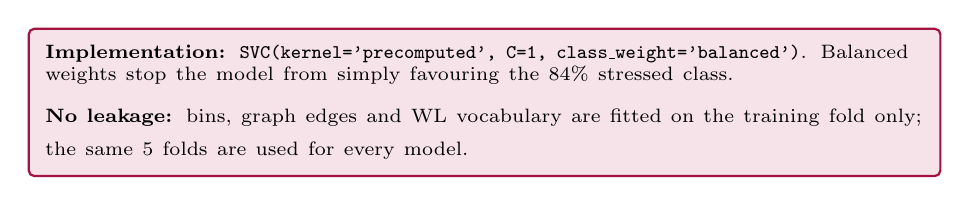
\begin{tikzpicture}
            \node[rectangle, draw=amritaMaroon, thick, fill=maroonSoft,
                  rounded corners=2pt, inner sep=6pt, text width=0.92\columnwidth] {
                \scriptsize\textbf{Implementation:} \texttt{SVC(kernel='precomputed', C=1, class\_weight='balanced')}. Balanced weights stop the model from simply favouring the 84\% stressed class.\\[3pt]
                \textbf{No leakage:} bins, graph edges and WL vocabulary are fitted on the training fold only; the same 5 folds are used for every model.
            };
        \end{tikzpicture}
    \end{columns}
\end{frame}


% ============================================================
% SLIDE: Model Evaluation & Performance Metrics
% ============================================================
\begin{frame}{Model Evaluation \& Performance Metrics}
    \framesubtitle{Evaluating the SVM via K-Fold Cross-Validation \cite{kohavi1995study}} % Replace with your BibTeX key

    % --- Section 1: K-Fold Cross-Validation Diagram ---
    {\normalsize\bfseries 1. K-Fold Cross-Validation \cite{kohavi1995study}} % Replace with your BibTeX key

    \vspace{0.15cm}
    \begin{center}
        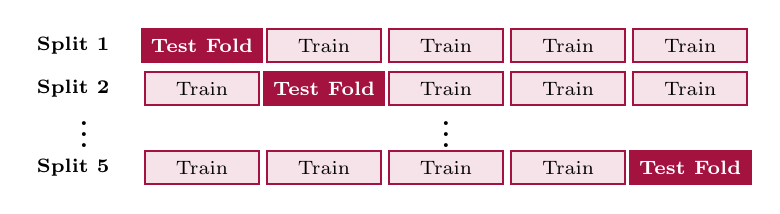
\begin{tikzpicture}[
            splitlbl/.style={font=\scriptsize\bfseries, anchor=east},
            trainbox/.style={rectangle, draw=amritaMaroon, thick, fill=maroonSoft,
                             minimum width=1.45cm, minimum height=0.42cm,
                             font=\scriptsize, text=black},
            testbox/.style={rectangle, draw=amritaMaroon, thick, fill=amritaMaroon,
                            minimum width=1.45cm, minimum height=0.42cm,
                            font=\scriptsize\bfseries, text=white}
        ]
            % Split 1
            \node[splitlbl] at (-0.3, 0) {Split 1};
            \node[testbox]  at (0.75, 0) {Test Fold};
            \node[trainbox] at (2.30, 0) {Train};
            \node[trainbox] at (3.85, 0) {Train};
            \node[trainbox] at (5.40, 0) {Train};
            \node[trainbox] at (6.95, 0) {Train};

            % Split 2
            \node[splitlbl] at (-0.3, -0.55) {Split 2};
            \node[trainbox] at (0.75, -0.55) {Train};
            \node[testbox]  at (2.30, -0.55) {Test Fold};
            \node[trainbox] at (3.85, -0.55) {Train};
            \node[trainbox] at (5.40, -0.55) {Train};
            \node[trainbox] at (6.95, -0.55) {Train};

            % Vertical Ellipses
            \node[font=\small\bfseries] at (-0.75, -1.02) {$\vdots$};
            \node[font=\small\bfseries] at (3.85,  -1.02) {$\vdots$};

            % Split 5
            \node[splitlbl] at (-0.3, -1.55) {Split 5};
            \node[trainbox] at (0.75, -1.55) {Train};
            \node[trainbox] at (2.30, -1.55) {Train};
            \node[trainbox] at (3.85, -1.55) {Train};
            \node[trainbox] at (5.40, -1.55) {Train};
            \node[testbox]  at (6.95, -1.55) {Test Fold};
        \end{tikzpicture}
    \end{center}

    \vspace{0.15cm}
    % --- Section 2: Calculating Metrics ---
    {\normalsize\bfseries 2. Calculating Metrics}\\[2pt]
    {\scriptsize Computed on each test fold, then averaged. $TP$ = stressed leaf called stressed; $TN$ = healthy leaf called healthy.}
    \vspace{0.05cm}
    \begin{columns}[T, onlytextwidth]
        \column{0.49\textwidth}
        \begin{itemize}\scriptsize
            \setlength{\itemsep}{1pt}
            \item \textbf{Accuracy} $= \frac{TP+TN}{\text{all leaves}}$
            \item \textbf{Precision} $= \frac{TP}{TP+FP}$
            \item \textbf{Recall} (stressed found) $= \frac{TP}{TP+FN}$
            \item \textbf{F1} $= \frac{2\,P\,R}{P+R}$
        \end{itemize}
        \column{0.49\textwidth}
        \begin{itemize}\scriptsize
            \setlength{\itemsep}{1pt}
            \item \textbf{\textcolor{amritaMaroon}{Macro-F1}} (main) $= \frac{F1_{\text{healthy}} + F1_{\text{stressed}}}{2}$
            \item \textbf{Balanced acc.} $= \frac{\text{stressed found} + \text{healthy found}}{2}$
            \item \textbf{Healthy found} (specificity) $= \frac{TN}{TN+FP}$
        \end{itemize}
        {\tiny Why: 84\% of leaves are stressed, so always answering ``stressed'' gets 83.8\% accuracy but only 0.456 macro-F1.}
    \end{columns}
\end{frame}

% % ============================================================
% % FRAME: Role Separation & Viva Explanation
% % ============================================================
% \begin{frame}{Role Separation: Methodology Architecture}
%     \framesubtitle{Clear functional division between pipeline components}

%     \begin{table}[]
%         \centering
%         \scriptsize
%         \begin{tabular}{p{3.2cm} p{6.8cm}}
%             \toprule
%             \textbf{Component} & \textbf{Core Function} \\
%             \midrule
%             38 Extracted Features & Quantify physical leaf morphology, color, texture, and regions. \\
%             Graph Construction & Defines structural topologies and inter-trait relationships. \\
%             WL Algorithm & Captures local and multi-hop subtree structures via relabeling. \\
%             WL Subtree Vector ($\Phi$) & High-dimensional numerical count of discovered graph subtrees. \\
%             WL Kernel ($K$) & Quantifies pairwise structural similarity between leaf graphs. \\
%             SVM Classifier & Learns the optimal maximum-margin hyperplane for stress labels. \\
%             \bottomrule
%         \end{tabular}
%     \end{table}

%     \vspace{0.25cm}
%     \begin{tikzpicture}
%         \node[rectangle, draw=amritaMaroon, very thick, fill=maroonSoft,
%               rounded corners=3pt, inner sep=7pt, text width=0.92\textwidth] {
%             \footnotesize
%             \textbf{Key Takeaway:} \textit{“WL extracts structural patterns from the feature graph, the kernel calculates similarity between those patterns, and the SVM uses these similarities to classify leaves as stressed or non-stressed.”}
%         };
%     \end{tikzpicture}
% \end{frame}

% % ============================================================
% % FRAME: Experimental Evaluation Setup
% % ============================================================
% \begin{frame}{Experimental Evaluation Configuration}
%     \framesubtitle{Comprehensive grid evaluation across topologies, depths, and folds}

%     \begin{columns}[c]
%         \column{0.50\textwidth}
%         \textbf{Evaluation Grid Dimensions}
%         \vspace{0.2cm}

%         \begin{itemize}\footnotesize
%             \item \textbf{5 Graph Topologies:}
%             \begin{itemize}\scriptsize
%                 \item Correlation Graph
%                 \item Feature-Similarity $k$-NN Graph
%                 \item Feature Family Graph
%                 \item Spatial / Regional Graph
%                 \item Hybrid Graph
%             \end{itemize}
%             \vspace{0.15cm}
%             \item \textbf{4 WL Subtree Heights:}
%             \begin{itemize}\scriptsize
%                 \item $h \in \{0, 1, 2, 3\}$
%             \end{itemize}
%             \vspace{0.15cm}
%             \item \textbf{Validation Protocol:}
%             \begin{itemize}\scriptsize
%                 \item Stratified 5-Fold Cross-Validation
%             \end{itemize}
%         \end{itemize}

%         \column{0.46\textwidth}
%         \centering
%         \begin{tikzpicture}[every node/.style={transform shape}]
%             \node[stepbox, fill=maroonSoft, minimum width=4.0cm] (m1) {\textbf{5 Graph Types}};
%             \node[stepbox, fill=maroonSoft, minimum width=4.0cm, below=0.25cm of m1] (m2) {\textbf{4 WL Heights ($h=0..3$)}};
%             \node[stepbox, fill=maroonSoft, minimum width=4.0cm, below=0.25cm of m2] (m3) {\textbf{5 Validation Folds}};
            
%             \node[stepbox, fill=amritaMaroon, text=white, minimum width=4.0cm, below=0.4cm of m3] (tot) {
%                 \textbf{Total Evaluations: 100} \\
%                 {\tiny $5 \times 4 \times 5 = 100\text{ Fold Experiments}$}
%             };

%             \draw[-{Latex[length=2mm]}, thick, draw=amritaMaroon] (m1) -- (m2);
%             \draw[-{Latex[length=2mm]}, thick, draw=amritaMaroon] (m2) -- (m3);
%             \draw[-{Latex[length=2mm]}, thick, draw=amritaMaroon] (m3) -- (tot);
%         \end{tikzpicture}
%     \end{columns}
% \end{frame}

% ============================================================
% FRAME: Model Evaluation (Testing on Folds)
% ============================================================


% % ============================================================
% % SLIDE 23: All 20 Configurations (Table 1)
% % ============================================================
% \begin{frame}{Configuration Performance}
%     \framesubtitle{All 20 configurations ranked by Macro-F1 (Primary Metric) across WL heights $h \in \{0,1,2,3\}$}

%     \begin{columns}[T, onlytextwidth]
%         % --- Left Column: Top 10 Ranked Configurations ---
%         \column{0.485\textwidth}
%         \centering
%         {\scriptsize\bfseries\textcolor{amritaMaroon}{Top 10 Configurations (Ranks \#1 -- \#10)}}\\[3pt]
%         \begin{table}
%             \centering
%             \tiny
%             \setlength{\tabcolsep}{3.5pt}
%             \renewcommand{\arraystretch}{1.28}
%             \begin{tabular}{@{}clrrrr@{}}
%                 \toprule
%                 \textbf{\#} & \textbf{Graph Type} & \textbf{$h$} & \textbf{Acc.} & \textbf{M-F1} & \textbf{W-F1} \\
%                 \midrule
%                 \textbf{\textcolor{amritaMaroon}{1}} & \textbf{\textcolor{amritaMaroon}{Hybrid}} & \textbf{3} & \textbf{0.8160} & \textbf{\textcolor{amritaMaroon}{0.6969}} & \textbf{0.8251} \\
%                 \textbf{2} & \textbf{Feature-Family} & 3 & 0.8092 & \textbf{0.6914} & 0.8201 \\
%                 \textbf{3} & \textbf{Hybrid} & 2 & 0.7971 & \textbf{0.6874} & 0.8124 \\
%                 4 & Feature-Family & 2 & 0.7891 & 0.6817 & 0.8065 \\
%                 5 & Feature-Similarity kNN & 3 & 0.7787 & 0.6737 & 0.7985 \\
%                 6 & Feature-Similarity kNN & 2 & 0.7620 & 0.6647 & 0.7865 \\
%                 7 & Hybrid & 1 & 0.7575 & 0.6591 & 0.7826 \\
%                 8 & Feature-Family & 1 & 0.7534 & 0.6557 & 0.7794 \\
%                 9 & Feature-Similarity kNN & 1 & 0.7237 & 0.6374 & 0.7567 \\
%                 10 & Correlation & 3 & 0.7094 & 0.6216 & 0.7445 \\
%                 \bottomrule
%             \end{tabular}
%         \end{table}

%         % --- Right Column: Remaining 10 Configurations + Callout ---
%         \column{0.485\textwidth}
%         \centering
%         {\scriptsize\bfseries\textcolor{inkGray}{Remaining Configurations (Ranks \#11 -- \#20)}}\\[3pt]
%         \begin{table}
%             \centering
%             \tiny
%             \setlength{\tabcolsep}{3.5pt}
%             \renewcommand{\arraystretch}{1.28}
%             \begin{tabular}{@{}clrrrr@{}}
%                 \toprule
%                 \textbf{\#} & \textbf{Graph Type} & \textbf{$h$} & \textbf{Acc.} & \textbf{M-F1} & \textbf{W-F1} \\
%                 \midrule
%                 11 & Spatial/Regional & 2 & 0.7064 & 0.6216 & 0.7424 \\
%                 12 & Spatial/Regional & 3 & 0.7082 & 0.6212 & 0.7437 \\
%                 13 & Spatial/Regional & 1 & 0.6987 & 0.6175 & 0.7363 \\
%                 14 & Correlation & 2 & 0.6996 & 0.6170 & 0.7369 \\
%                 15 & Correlation & 1 & 0.6914 & 0.6117 & 0.7303 \\
%                 16 & Feature-Similarity kNN & 0 & 0.6747 & 0.6007 & 0.7167 \\
%                 17 & Feature-Family & 0 & 0.6747 & 0.6007 & 0.7167 \\
%                 18 & Hybrid & 0 & 0.6747 & 0.6007 & 0.7167 \\
%                 19 & Correlation & 0 & 0.6747 & 0.6007 & 0.7167 \\
%                 20 & Spatial/Regional & 0 & 0.6747 & 0.6007 & 0.7167 \\
%                 \bottomrule
%             \end{tabular}
%         \end{table}
%     \end{columns}

%     \vspace{0.18cm}
%     \begin{center}
%         \begin{tikzpicture}
%             \node[rectangle, draw=amritaMaroon, thick, fill=maroonSoft,
%                   rounded corners=3pt, inner sep=5.5pt, text width=0.95\textwidth, align=center] {
%                 {\scriptsize \textbf{\textcolor{amritaMaroon}{Key Pattern:}} All $h=0$ baselines tie at \textbf{0.6007 Macro-F1} (isolated node counts only); multi-hop structural aggregation ($h=3$) on the \textbf{Hybrid} graph yields a \textbf{+9.62\% Macro-F1} and \textbf{+14.13\% Accuracy} gain.}
%             };
%         \end{tikzpicture}
%     \end{center}
% \end{frame}

% % ============================================================
% % FRAME: All 22 Configurations (Table 1)
% % ============================================================
% % ============================================================
% % FRAME: All 22 Configurations (Table 1)
% % ============================================================
% % ============================================================
% % FRAME: All 20 Configurations (Table 1)
% % ============================================================
% % ============================================================
% % FRAME: All 20 Configurations (Table 1)
% % ============================================================


% ============================================================
% RESULTS 1: Graph topology matters (research question)
% ============================================================
\begin{frame}{Results 1: Graph Construction Changes WL Performance}
    \framesubtitle{Healthy vs stressed, all 4,387 leaves, same 5 folds: best macro-F1 per graph type}

    \begin{columns}[T, onlytextwidth]
        \column{0.58\textwidth}
        \centering
        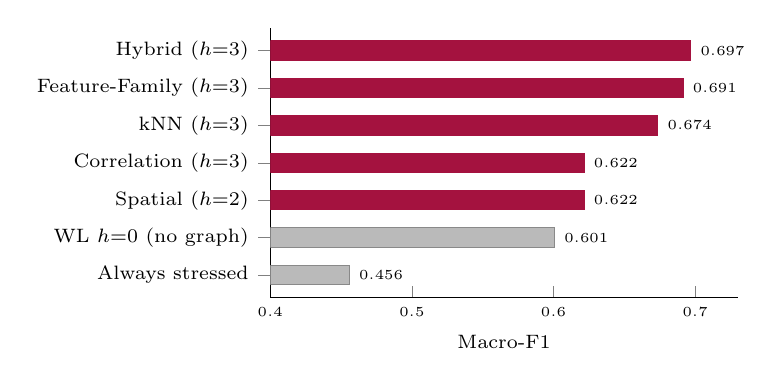
\begin{tikzpicture}
            \begin{axis}[
                xbar, width=0.62\linewidth, height=5.0cm,
                xmin=0.40, xmax=0.73,
                ytick={0,1,2,3,4,5,6}, bar shift=0pt, ymin=-0.6, ymax=6.6,
                yticklabels={Always stressed, WL $h{=}0$ (no graph), Spatial ($h{=}2$), Correlation ($h{=}3$), kNN ($h{=}3$), Feature-Family ($h{=}3$), Hybrid ($h{=}3$)},
                y tick label style={font=\scriptsize},
                x tick label style={font=\tiny, /pgf/number format/fixed},
                xlabel={\scriptsize Macro-F1}, bar width=7pt, 
                nodes near coords, nodes near coords style={font=\tiny, /pgf/number format/fixed, /pgf/number format/precision=3},
                axis x line*=bottom, axis y line*=left,
            ]
                \addplot[fill=amritaMaroon, draw=amritaMaroon] coordinates {
                    (0.6969,6) (0.6914,5) (0.6737,4)
                    (0.6216,3) (0.6216,2)
                };
                \addplot[fill=inkGray!35, draw=inkGray!60] coordinates {
                    (0.6007,1) (0.4558,0)
                };
            \end{axis}
        \end{tikzpicture}

        \column{0.39\textwidth}
        {\scriptsize\bfseries\textcolor{amritaMaroon}{Deeper WL helps (Hybrid graph)}}\\[2pt]
        \centering
        \scriptsize
        \renewcommand{\arraystretch}{1.15}
        \begin{tabular}{@{}c c c@{}}
            \toprule
            \textbf{$h$} & \textbf{Macro-F1} & \textbf{Accuracy} \\
            \midrule
            0 & 0.601 & 0.675 \\
            1 & 0.659 & 0.758 \\
            2 & 0.687 & 0.797 \\
            \textbf{3} & \textbf{\textcolor{amritaMaroon}{0.697}} & \textbf{0.816} \\
            \bottomrule
        \end{tabular}

        \vspace{0.2cm}
        \raggedright
        {\scriptsize At $h{=}0$ every graph scores the same (0.601): the gain comes only from the edges WL follows.}
    \end{columns}

    \vspace{0.12cm}
    \centering
    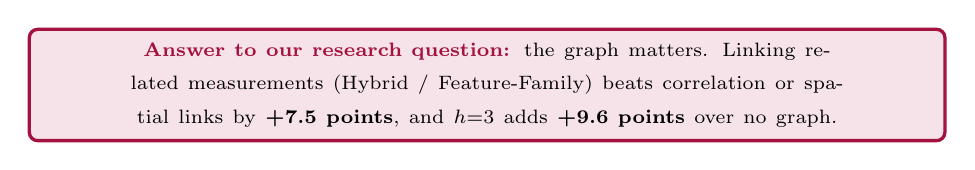
\begin{tikzpicture}
        \node[notebox, inner sep=5pt, text width=0.93\textwidth, align=center] {
            \scriptsize \textbf{\textcolor{amritaMaroon}{Answer to our research question:}} the graph matters. Linking related measurements
            (Hybrid / Feature-Family) beats correlation or spatial links by \textbf{+7.5 points}, and $h{=}3$ adds \textbf{+9.6 points} over no graph.
        };
    \end{tikzpicture}
\end{frame}

% ============================================================
% RESULTS 2: Fair benchmark incl. CNN (accuracy, robustness, speed)
% ============================================================
\begin{frame}{Results 2: Fair Benchmark Against Baselines and a CNN}
    \framesubtitle{Full pipeline (find the crop, then that crop's stress model), same 5 folds for every model}

    \centering
    \scriptsize
    \setlength{\tabcolsep}{3.5pt}
    \renewcommand{\arraystretch}{1.18}
    \begin{tabular}{@{}l c c c c c@{}}
        \toprule
        \textbf{Model} & \textbf{Macro-F1} & \textbf{Bal.\ acc.} & \textbf{Healthy found} & \textbf{F1 change, altered photo} & \textbf{Time / photo} \\
        \midrule
        CNN EfficientNet-B0 (frozen) & \textbf{0.739} & 0.756 & 62\% & $\pm$0.00 & \textbf{0.14 s} \\
        Extra Trees (tuned) & 0.729 & 0.730 & 55\% & $-$0.10 & 1.07 s \\
        Gradient Boosting (tuned) & 0.721 & 0.725 & 55\% & $-$0.08 & 1.08 s \\
        \rowcolor{maroonSoft}
        \textbf{\textcolor{amritaMaroon}{WL + SVM (ours, best)}} & \textbf{0.706} & 0.723 & 57\% & \textbf{$-$0.05} & 1.08 s \\
        \rowcolor{maroonSoft}
        WL + SVM (ours, tuned) & 0.683 & 0.702 & 54\% & -- & 1.08 s \\
        Random Forest (default) & 0.682 & 0.645 & 31\% & $-$0.18 & 1.07 s \\
        \midrule
        Always answers ``stressed'' & 0.456 & 0.500 & 0\% & -- & -- \\
        \bottomrule
    \end{tabular}

    \vspace{0.05cm}
    {\tiny Baselines: 13 measurement-based models (e.g.\ Extra Trees \cite{geurts2006extremely}) and 2 frozen ImageNet CNNs (EfficientNet-B0 \cite{tan2019efficientnet}). Tuned = settings chosen inside each training fold only (nested CV \cite{varma2006bias}). Photo altered = 240 photos $\times$ 7 changes (darker, brighter, warm light, blur, strong JPEG, noise, half resolution).
    Time includes finding the leaf in the full 3,024 px photo; the CNN looks at a 224 px copy.}

    \vspace{0.15cm}
    \begin{columns}[T, onlytextwidth]
        \column{0.32\textwidth}
        
\begin{tikzpicture}
            \node[notebox, inner sep=5pt, text width=0.88\columnwidth] {
                {\tiny\bfseries\textcolor{amritaMaroon}{ACCURACY}}\\
                {\scriptsize CNN is best; WL is \textbf{competitive}, 3.3 points behind.}
            };
        \end{tikzpicture}
        \column{0.32\textwidth}
        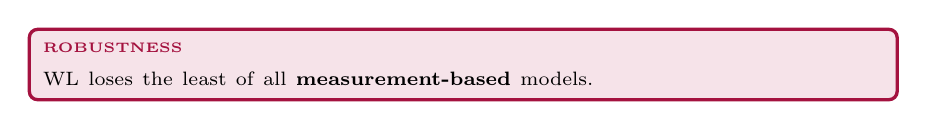
\begin{tikzpicture}
            \node[notebox, inner sep=5pt, text width=0.88\columnwidth] {
                {\tiny\bfseries\textcolor{amritaMaroon}{ROBUSTNESS}}\\
                {\scriptsize WL loses the least of all \textbf{measurement-based} models.}
            };
        \end{tikzpicture}
        \column{0.32\textwidth}
        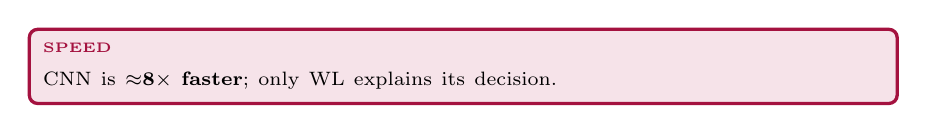
\begin{tikzpicture}
            \node[notebox, inner sep=5pt, text width=0.88\columnwidth] {
                {\tiny\bfseries\textcolor{amritaMaroon}{SPEED}}\\
                {\scriptsize CNN is $\approx$\textbf{8$\times$ faster}; only WL explains its decision.}
            };
        \end{tikzpicture}
    \end{columns}
\end{frame}

% ============================================================
% RESULTS 3: Where WL stands out (second opinion)
% ============================================================
\begin{frame}{Results 3: Where WL Stands Out, a Second Opinion Farmers Can Trust}
    \framesubtitle{CNN decides, WL checks and explains (all 4,387 leaves, held-out folds)}

    \begin{columns}[T, onlytextwidth]
        \column{0.53\textwidth}
        \small
        \renewcommand{\arraystretch}{1.2}
        \begin{tabular}{@{}l c c@{}}
            \toprule
            & \textbf{Leaves} & \textbf{CNN correct} \\
            \midrule
            \textcolor{green!50!black}{\textbf{$\bullet$ CNN and WL agree}} & 83\% & \textbf{91\%} \\
            \textcolor{orange!90!black}{\textbf{$\bullet$ CNN and WL disagree}} & 17\% & 56\% \\
            \midrule
            CNN alone (all leaves) & 100\% & 85\% \\
            \bottomrule
        \end{tabular}

        \vspace{0.3cm}
        
\begin{tikzpicture}
            \node[rectangle, draw=amritaMaroon, very thick, fill=amritaMaroon, text=white,
                  rounded corners=4pt, inner sep=6pt, text width=0.92\columnwidth, align=left] {
                {\scriptsize Disagreement flags only \textbf{17\%} of leaves but holds \textbf{51\%} of all CNN mistakes.
                The CNN's own confidence catches \textbf{44\%} when flagging the same number of leaves.}
            };
        \end{tikzpicture}

        \column{0.43\textwidth}
        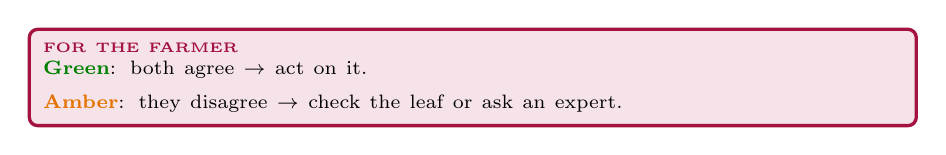
\begin{tikzpicture}
            \node[notebox, inner sep=5pt, text width=0.9\columnwidth] {
                {\tiny\bfseries\textcolor{amritaMaroon}{FOR THE FARMER}}\\
                {\scriptsize \textcolor{green!50!black}{\textbf{Green}}: both agree $\rightarrow$ act on it.\\
                \textcolor{orange!90!black}{\textbf{Amber}}: they disagree $\rightarrow$ check the leaf or ask an expert.}
            };
        \end{tikzpicture}

        \vspace{0.12cm}
        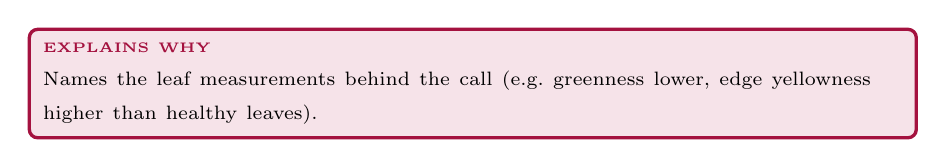
\begin{tikzpicture}
            \node[notebox, inner sep=5pt, text width=0.9\columnwidth] {
                {\tiny\bfseries\textcolor{amritaMaroon}{EXPLAINS WHY}}\\
                {\scriptsize Names the leaf measurements behind the call (e.g.\ greenness lower, edge yellowness higher than healthy leaves).}
            };
        \end{tikzpicture}

        \vspace{0.12cm}
        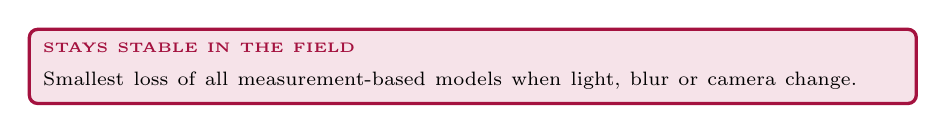
\begin{tikzpicture}
            \node[notebox, inner sep=5pt, text width=0.9\columnwidth] {
                {\tiny\bfseries\textcolor{amritaMaroon}{STAYS STABLE IN THE FIELD}}\\
                {\scriptsize Smallest loss of all measurement-based models when light, blur or camera change.}
            };
        \end{tikzpicture}
    \end{columns}

    \vspace{0.1cm}
    \centering
    {\tiny Tree models give a similar warning (53--59\%), but none explains itself in leaf terms or is as stable.}
\end{frame}

% ============================================================
% SLIDE 24: Crop Subgroup Performance (Table 3)
% ============================================================
\begin{frame}{Crop Subgroup Performance}
    \framesubtitle{The single Hybrid ($h = 3$) WL model, split by crop (5-fold CV, all 4,387 leaves)}

    \begin{columns}[T, onlytextwidth]
        \column{0.60\textwidth}
        \centering
        \scriptsize
        \setlength{\tabcolsep}{3.2pt}
        \renewcommand{\arraystretch}{1.22}
        \begin{tabular}{@{}l r r c c c@{}}
            \toprule
            \textbf{Crop} & \textbf{Leaves} & \textbf{Healthy} & \textbf{Macro-F1} & \textbf{Bal.\ acc.} & \textbf{Healthy found} \\
            \midrule
            \textbf{\textcolor{amritaMaroon}{Snake gourd}} & 452 & 58 & \textbf{\textcolor{amritaMaroon}{0.729}} & 0.687 & 40\% \\
            \textbf{Tomato} & 580 & 184 & \textbf{0.727} & 0.758 & \textbf{80\%} \\
            \textbf{Cucumber} & 240 & 34 & \textbf{0.722} & \textbf{0.780} & 71\% \\
            Eggplant & 662 & 91 & 0.668 & 0.690 & 51\% \\
            Bitter gourd & 742 & 173 & 0.655 & 0.688 & 64\% \\
            Ash gourd & 996 & 83 & 0.652 & 0.676 & 43\% \\
            Bottle gourd & 332 & 31 & 0.649 & 0.608 & 23\% \\
            Ridge gourd & 383 & 59 & 0.576 & 0.588 & 36\% \\
            \midrule
            \textbf{All crops} & 4,387 & 713 & \textbf{0.697} & 0.722 & 58\% \\
            {\tiny Always ``stressed''} & & & {\tiny 0.41--0.48} & {\tiny 0.500} & {\tiny 0\%} \\
            \bottomrule
        \end{tabular}

        \column{0.37\textwidth}
        
\begin{tikzpicture}
            \node[rectangle, draw=amritaMaroon, very thick, fill=amritaMaroon, text=white,
                  rounded corners=4pt, inner sep=6pt, text width=0.92\columnwidth, align=left] {
                {\tiny\bfseries\textcolor{maroonSoft}{MOST BALANCED}}\\[2pt]
                {\small\bfseries Tomato \& Cucumber}\\[2pt]
                {\scriptsize Find \textbf{71--80\%} of healthy leaves.}
            };
        \end{tikzpicture}

        \vspace{0.12cm}
        
\begin{tikzpicture}
            \node[notebox, inner sep=5pt, text width=0.92\columnwidth] {
                {\tiny\bfseries\textcolor{amritaMaroon}{HIGH ACCURACY CAN MISLEAD}}\\[1pt]
                {\scriptsize Bottle gourd: 92\% accuracy, but finds only \textbf{23\%} of its healthy leaves.}
            };
        \end{tikzpicture}

        \vspace{0.12cm}
        \begin{tikzpicture}
            \node[notebox, inner sep=5pt, text width=0.92\columnwidth] {
                {\tiny\bfseries\textcolor{amritaMaroon}{WHY SOME CROPS ARE HARDER}}\\[1pt]
                {\scriptsize Few healthy photos (ridge, bottle, ash gourd), so ``healthy'' is learned poorly.}
            };
        \end{tikzpicture}
    \end{columns}
\end{frame}

% ============================================================
% FRAME: All Metrics Graph
% ============================================================
% ============================================================
% FRAME: All Metrics Graph
% ============================================================
% \begin{frame}{Performance Across All Metrics}
%     \framesubtitle{Comparing Accuracy, F1-Scores, and Balanced Metrics}
%     \begin{center}
%         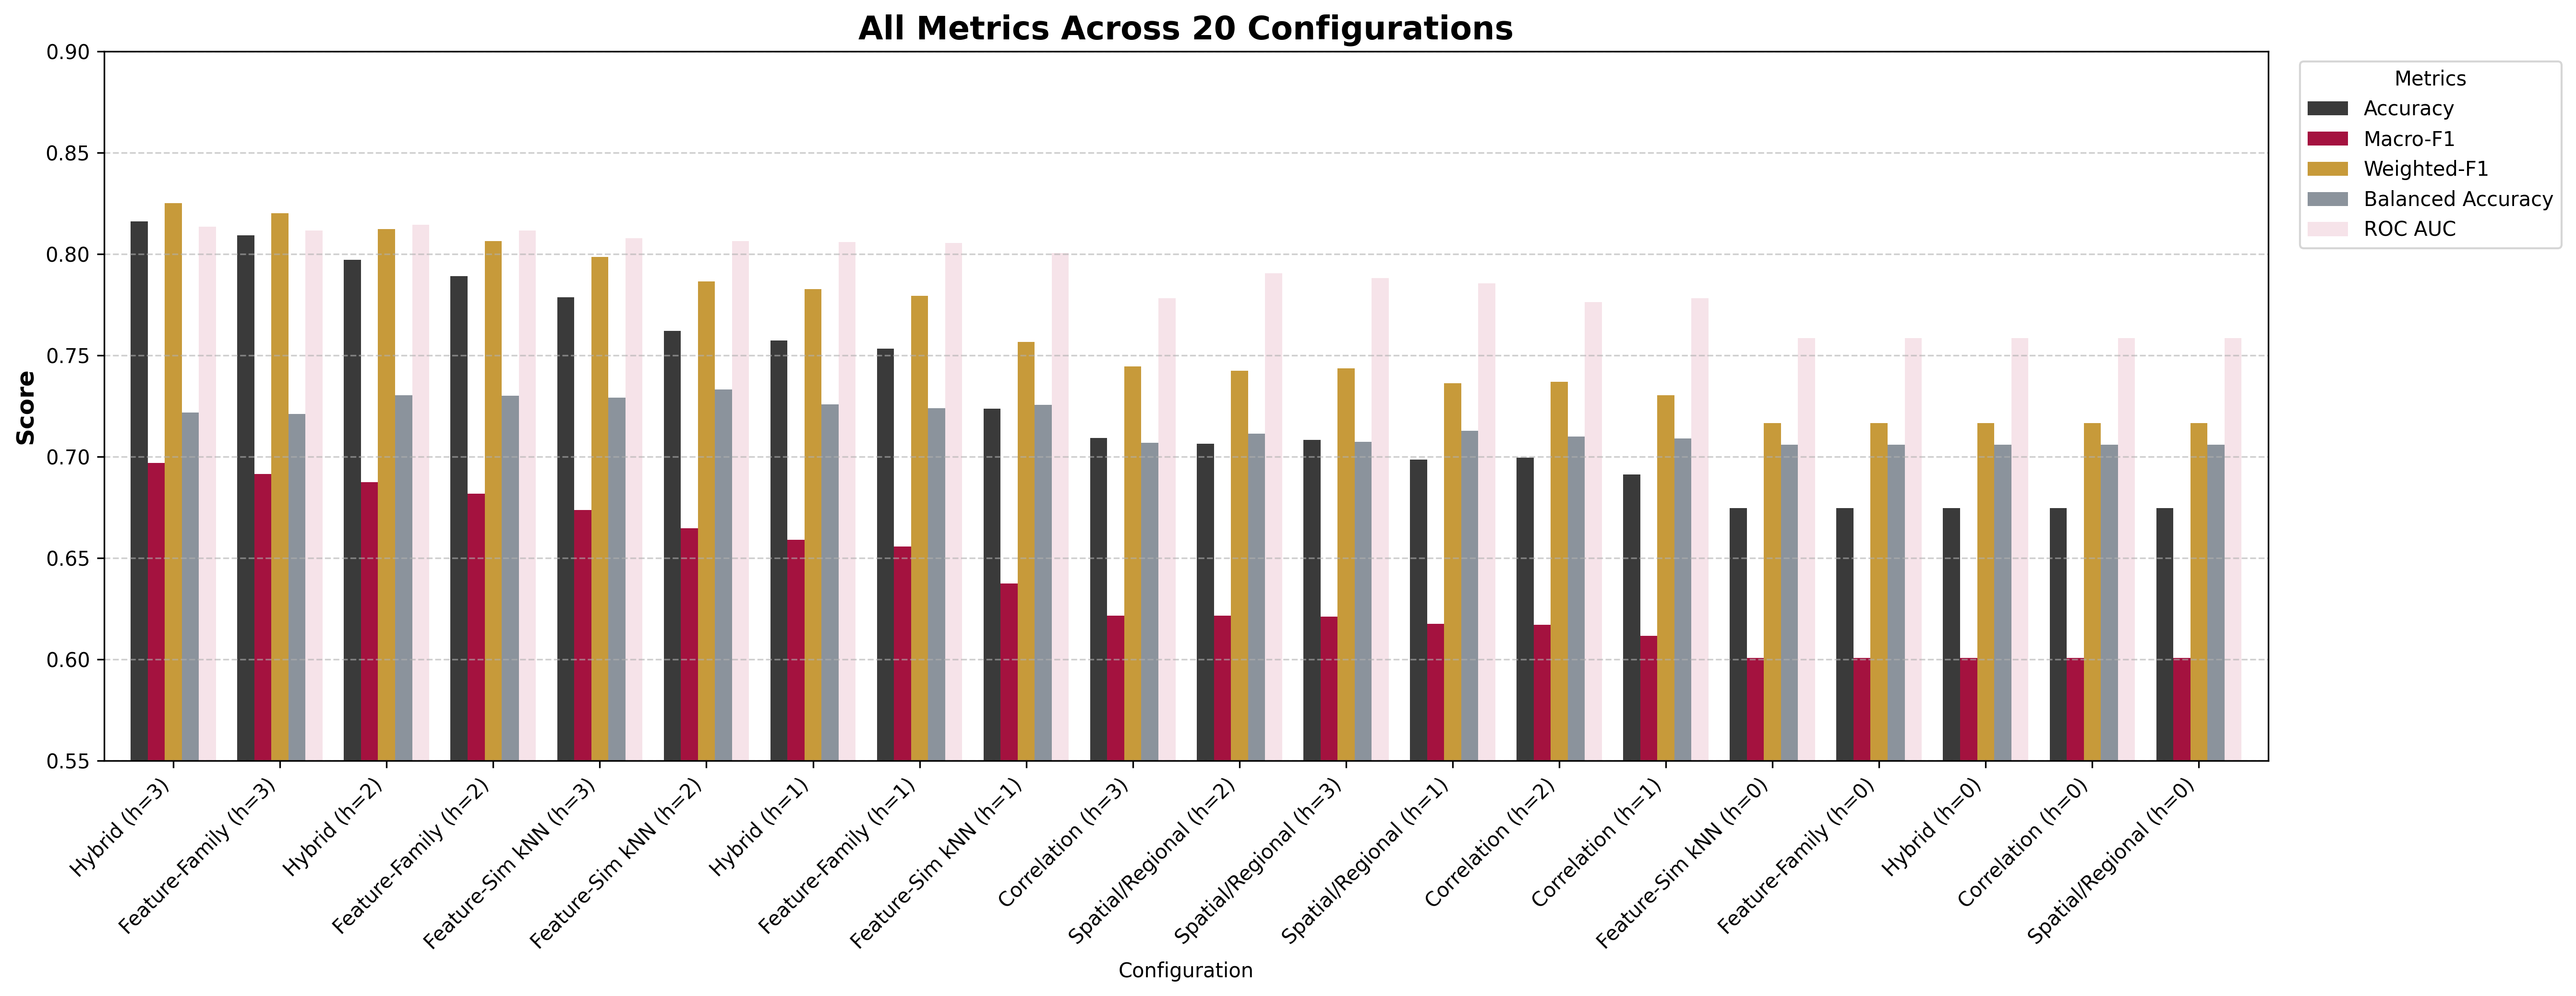
\includegraphics[width=\textwidth, height=0.8\textheight, keepaspectratio]{results_all_metrics.png}
%     \end{center}
% \end{frame}
% % ============================================================
% % FRAME: Side-by-Side Images (one.png & two.png)
% % ============================================================
% \begin{frame}{Additional Results}
%     \begin{columns}[onlytextwidth, c]
%         \column{0.49\textwidth}
%         \centering
%         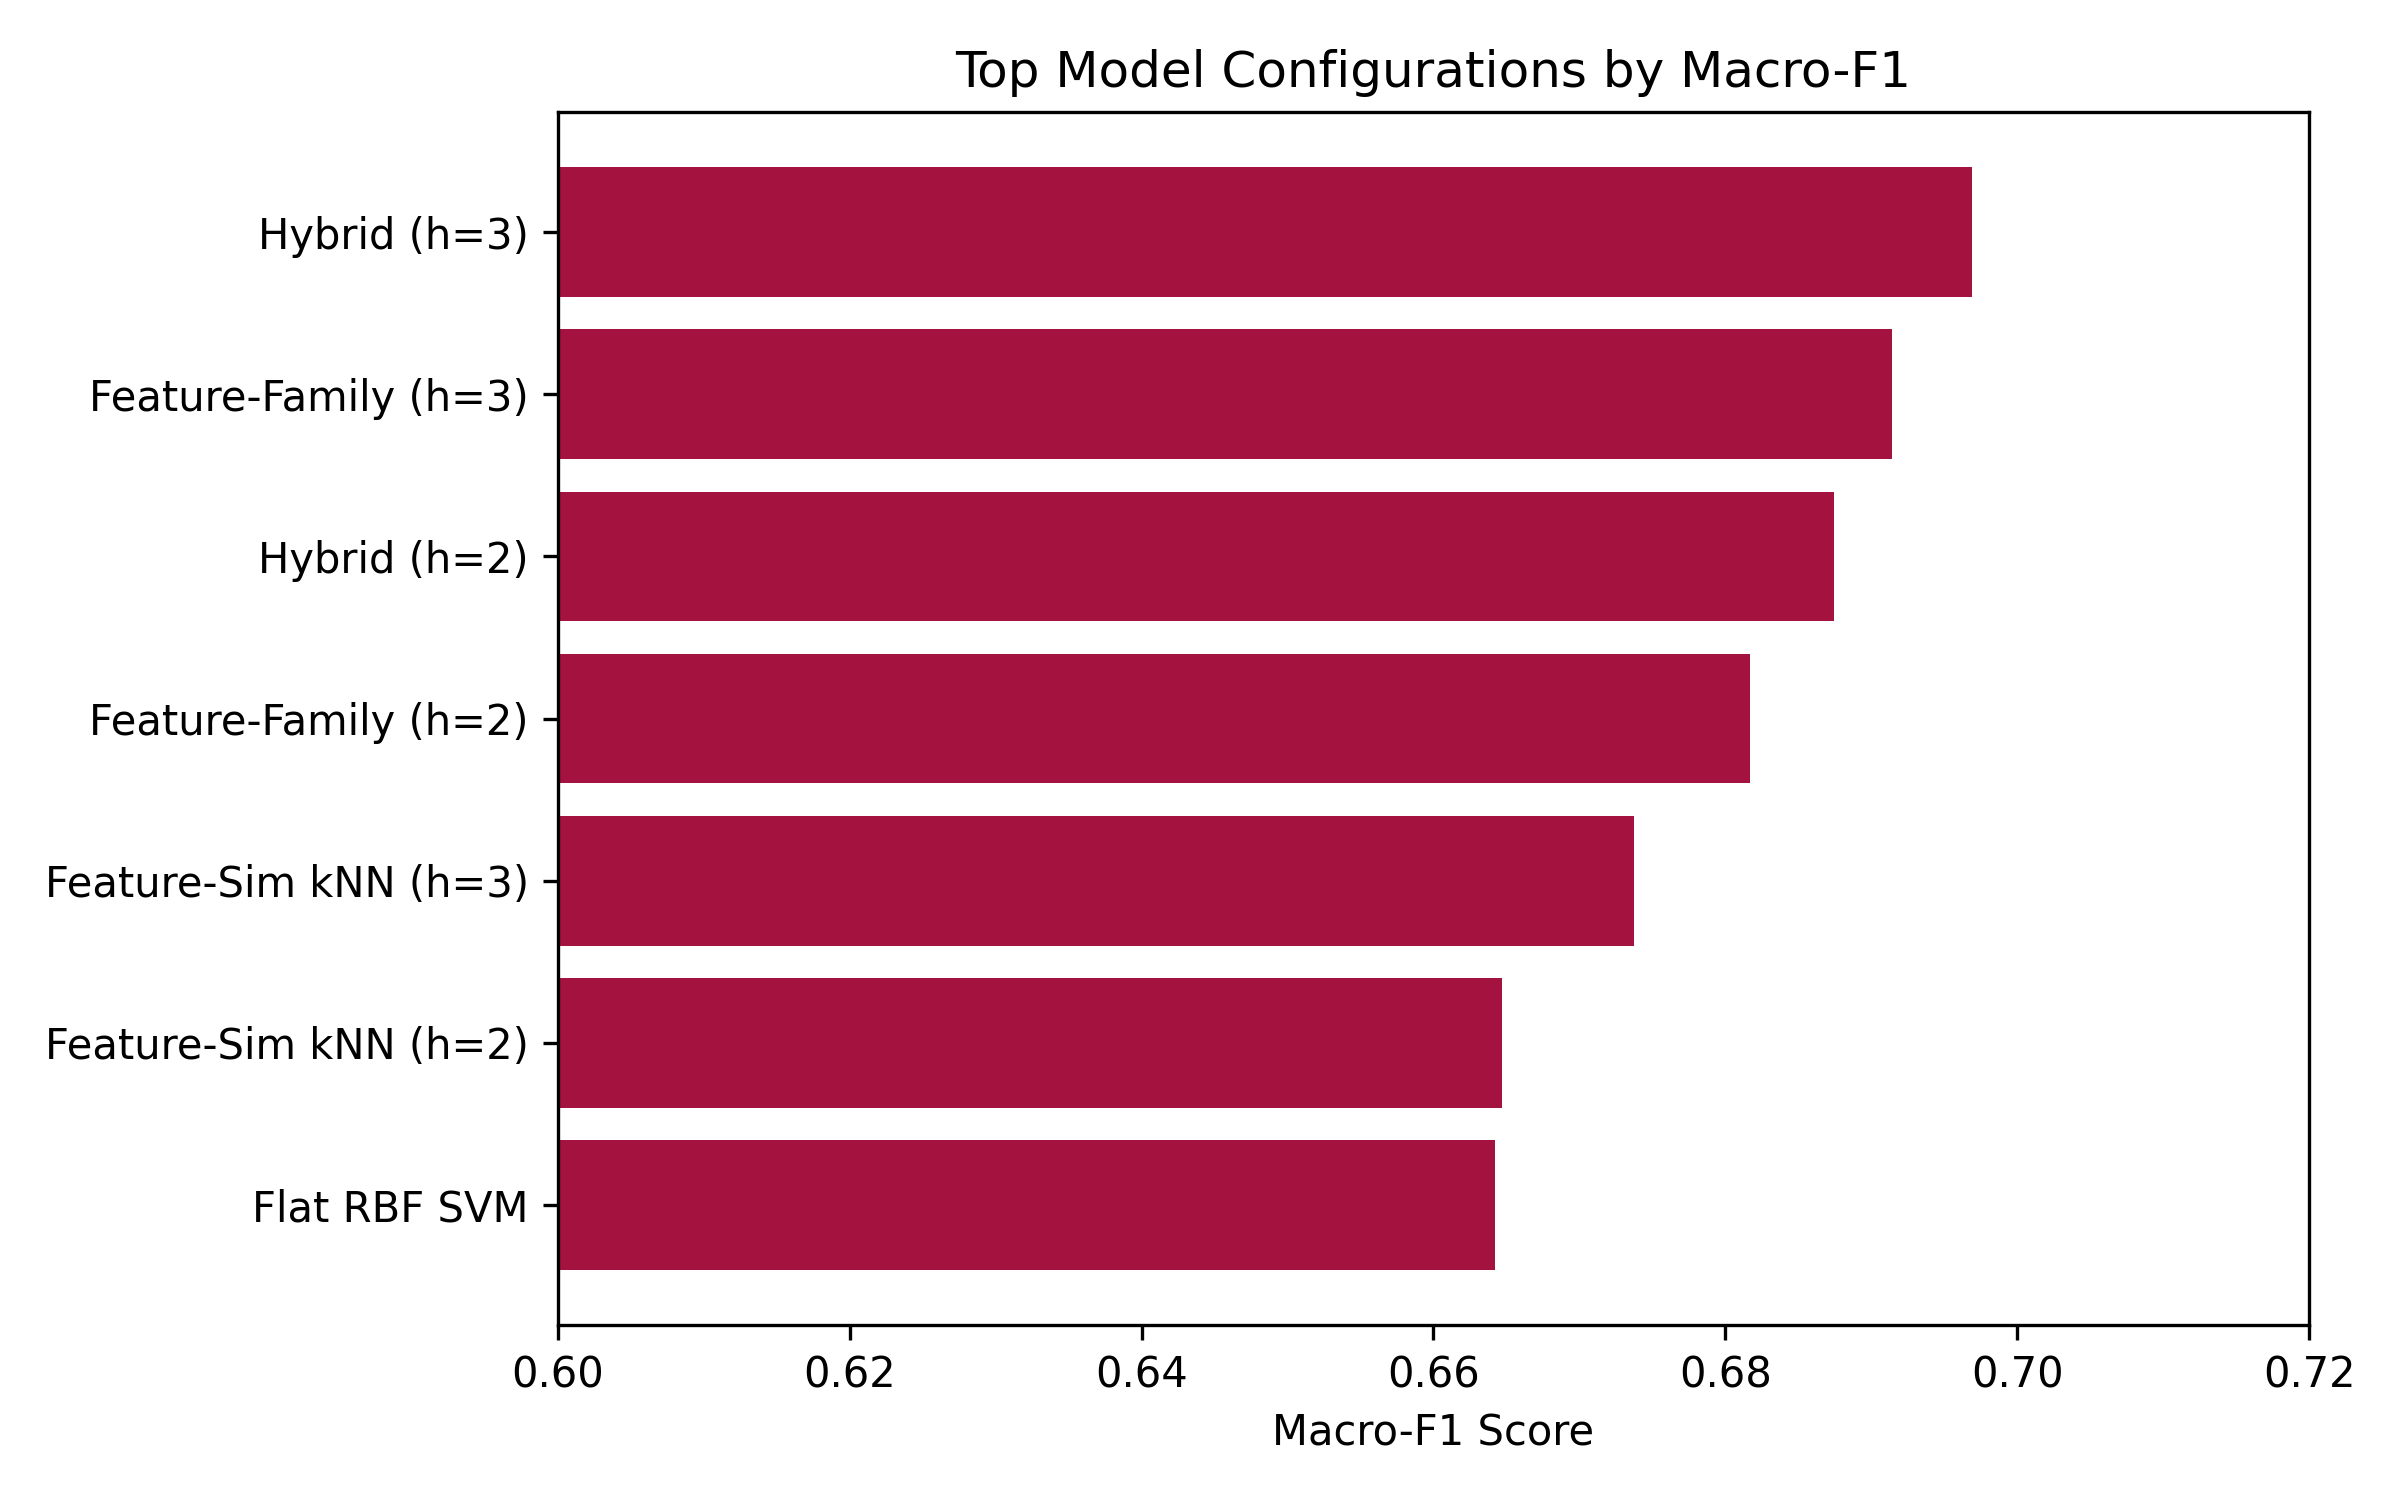
\includegraphics[width=\linewidth]{one.png}
        
%         \column{0.49\textwidth}
%         \centering
%         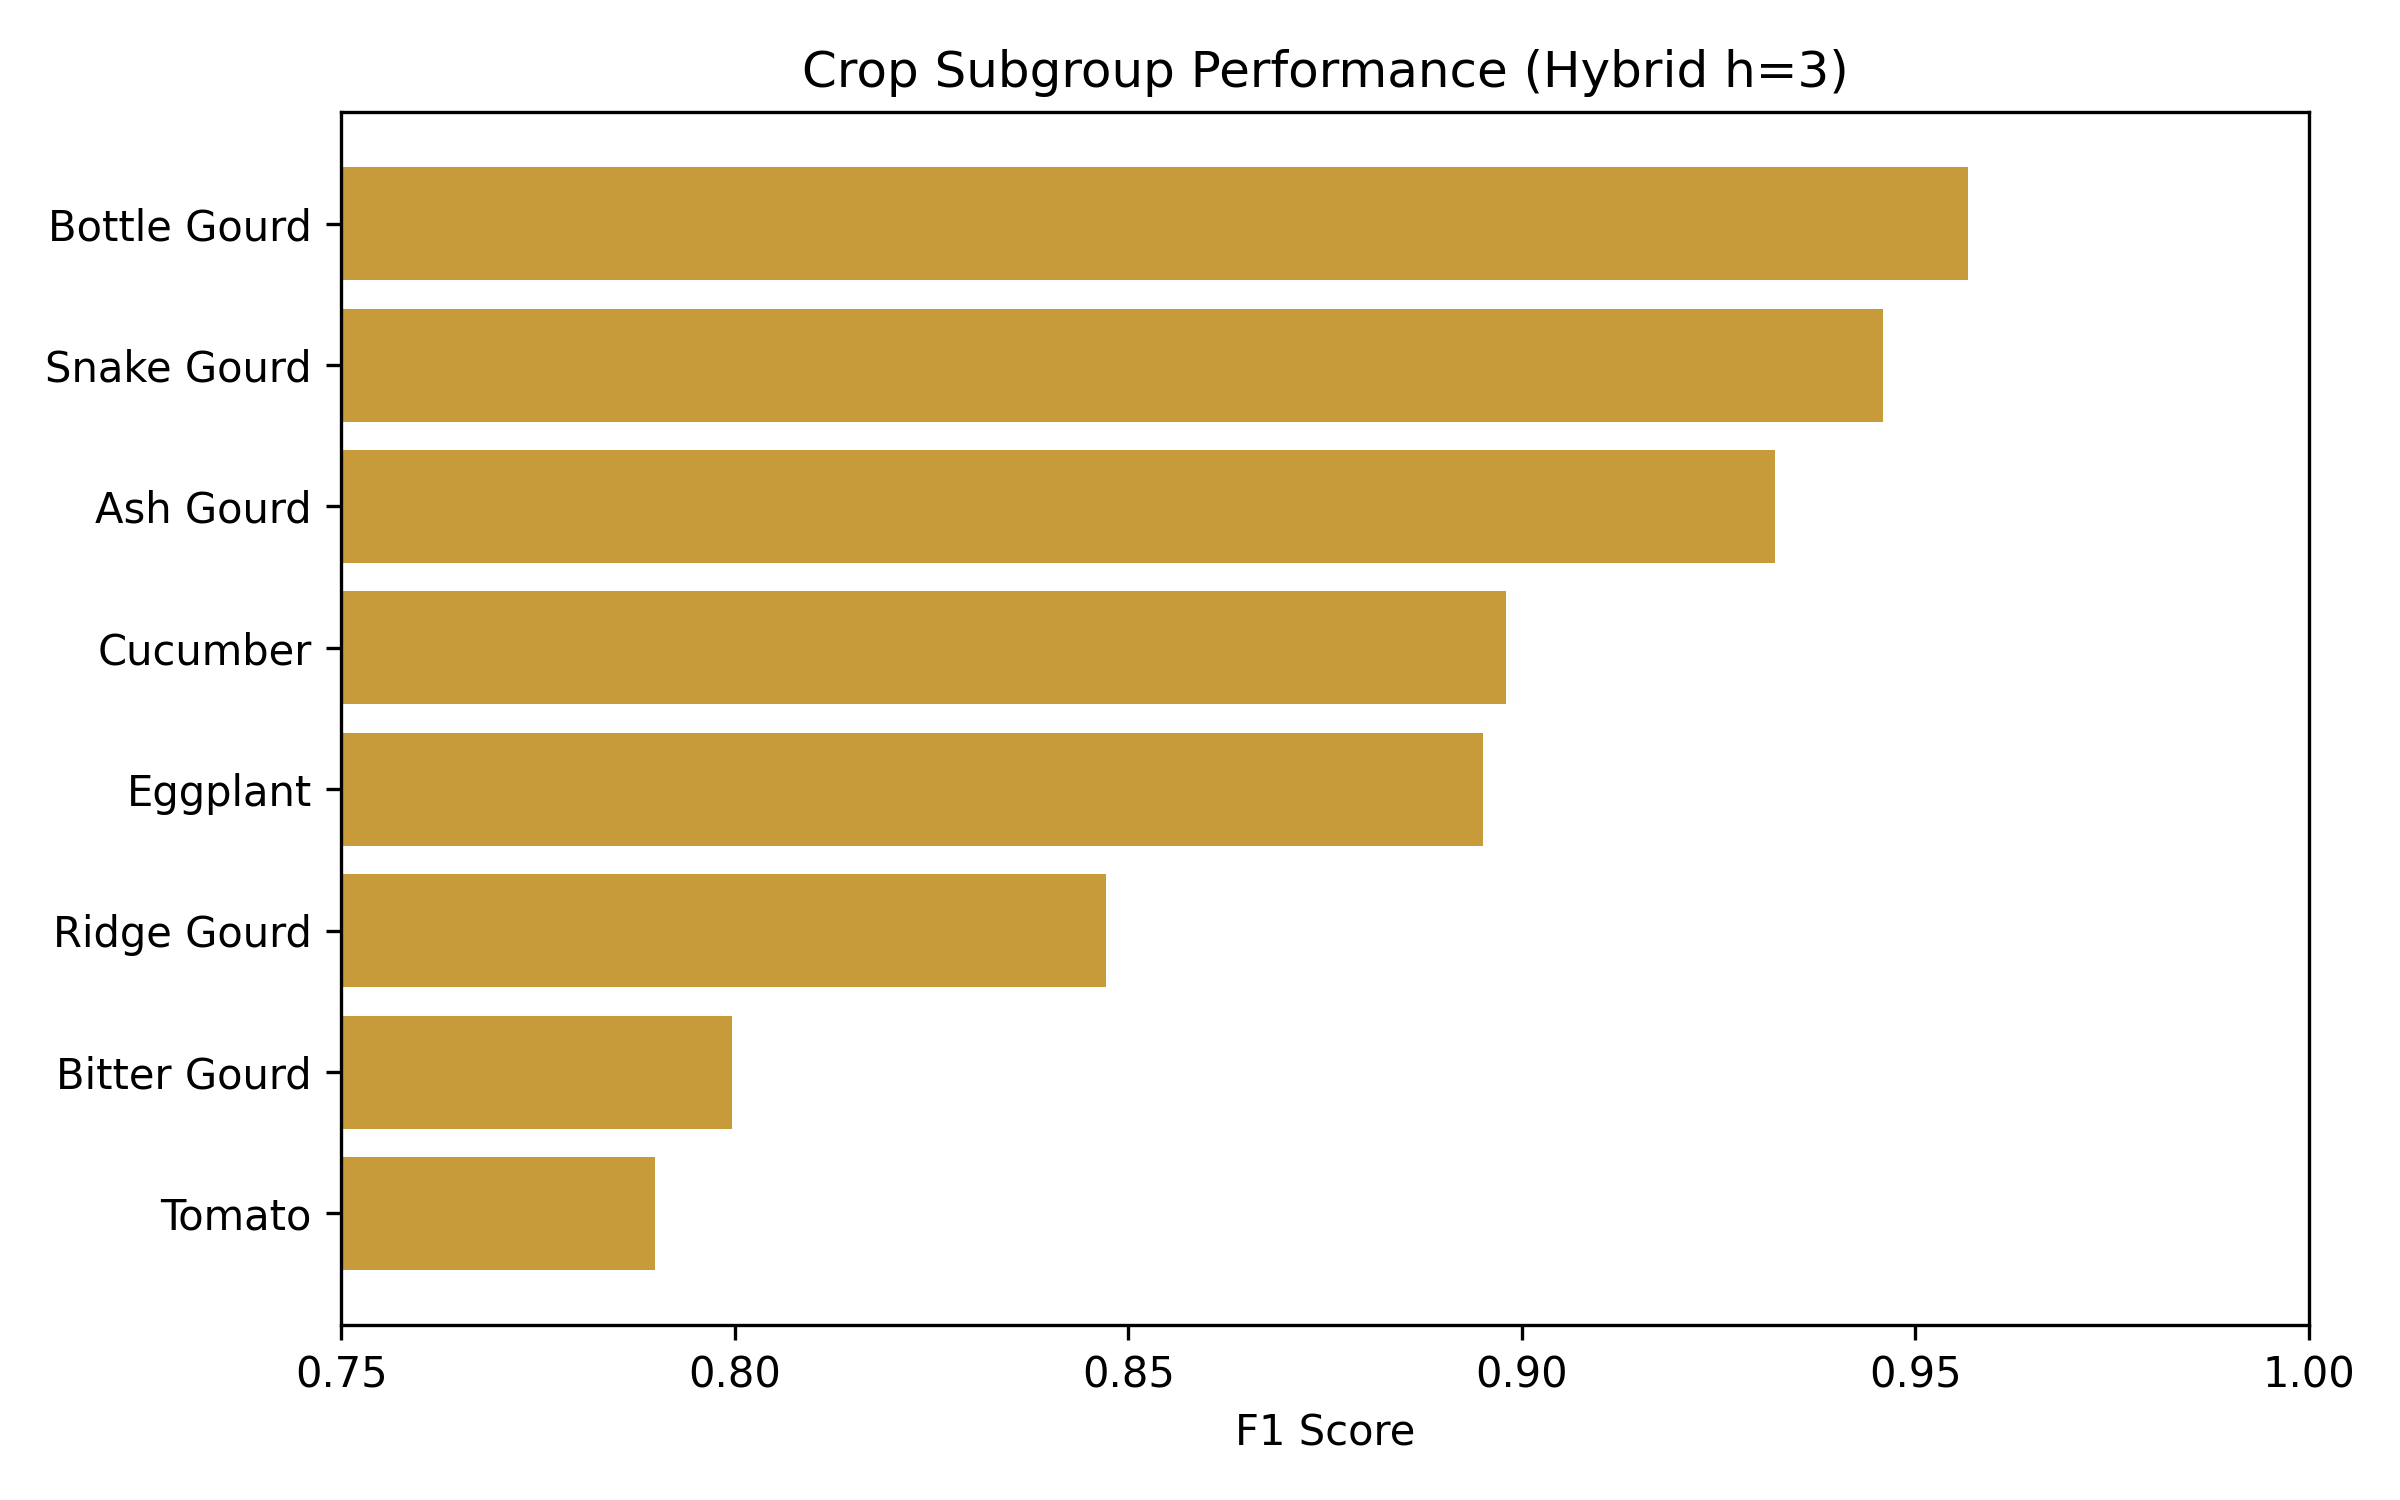
\includegraphics[width=\linewidth]{two.png}
%     \end{columns}
% \end{frame}
% ============================================================
% FRAME: Key Findings
% ============================================================
% \begin{frame}{Key Findings}
%     \framesubtitle{Effect of graph representation on WL kernel classification}

%     \begin{itemize}\small

%         % \item \textbf{Graph representation affects WL performance.}\\
%         % Different graph construction strategies produced clearly different
%         % classification results.

%         \vspace{0.15cm}

%         \item \textbf{Hybrid Graph + WL $h=3$ achieved the best overall performance.}\\
%         Macro-F1 = \textbf{0.6969}, Accuracy = \textbf{0.8160}.

%         \vspace{0.15cm}

%         \item \textbf{WL representation outperformed the flat baselines on Macro-F1.}\\
%         Hybrid $h=3$: \textbf{0.6969}
%         \quad vs. RBF-SVM: 0.6642
%         \quad vs. RF: 0.6522.

%         \vspace{0.15cm}

%         \item \textbf{Higher WL heights generally improved performance.}\\
%         $h=3$ was the best height for Correlation, Feature-Family,
%         Feature-Similarity kNN and Hybrid graphs; Spatial/Regional peaked at $h=2$.

%         \vspace{0.15cm}

%         \item \textbf{Performance varies across crops.}\\
%         With the fixed Hybrid $h=3$ model, F1 ranged from
%         \textbf{0.790 (Tomato)} to \textbf{0.957 (Bottle gourd)}.

%     \end{itemize}

%     \vspace{0.15cm}

%     % \begin{tikzpicture}
%     %     \node[rectangle, draw=amritaMaroon, thick, fill=maroonSoft,
%     %           rounded corners=2pt, inner sep=6pt,
%     %           text width=0.92\textwidth] {
%     %         \centering
%     %         \footnotesize\textbf{Key Research Finding:}
%     %         The choice of graph topology has a measurable impact on
%     %         the effectiveness of the Weisfeiler--Lehman kernel.
%     %     };
%     % \end{tikzpicture}

% \end{frame}

% \section{Technical Enrichment}
% \begin{frame}{4. Technical Enrichment Activity Choices}
%     \framesubtitle{Professional Online Certification Details}
%     \begin{itemize}
%         \item \textbf{Individual MOOC / Online Certification Selection:}
%     \end{itemize}
%     \vspace{-0.1cm}
%     \begin{table}
%         \centering
%         \footnotesize
%         \renewcommand{\arraystretch}{1.15}
%         \begin{tabular}{|c|p{2.8cm}|p{5.0cm}|p{2.3cm}|c|}
%             \hline
%             \textbf{S.No} & \textbf{Student Name} & \textbf{Chosen MOOC / Course Title} & \textbf{Platform} & \textbf{Hours} \\
%             \hline
%             1 & Vishnu   & [Supervised Machine Learning: Regression and Classification] & Coursera & 14 Hrs \\
%             \hline
%             2 & Vamsidhar & [Machine Learning and AI: Support Vector Machines in Python] & Udemy & 12 Hrs \\
%             \hline
%             3 & Bharath Bala & [IBM Machine Learning and AI: Support Vector Machines in Python] &  Coursera & 12 Hrs \\
%             \hline
%             4 & Sandeep M & [Introduction to Computer Vision and Image Processing] & Coursera & 16 Hrs \\
%             \hline
%              5 & Prakash CH & [Machine Learning in Drug Discovery and Cheminformatics] & Udemy & 12 Hrs \\
%             \hline
%         \end{tabular}
%     \end{table}
%     \vspace{0.15cm}
%     % \begin{itemize}
%     %     \item {\scriptsize \textbf{Requirement:} Each student must complete one approved 10--20 hour online certification from a recognized platform (Coursera, NPTEL, edX, etc.) relevant to the project.}
%     % \end{itemize}
% \end{frame}

% ============================================================
% FRAME: References
% ============================================================

% ============================================================
% SLIDE: Feature Application
% ============================================================
\begin{frame}{Application: PlantCare AI}
    \framesubtitle{Our web app turns the research into a tool a farmer can use (live demo next)}

    \centering
    \begin{tikzpicture}[>=Latex]
        \tikzset{appstep/.style={rectangle, draw=amritaMaroon, thick, fill=maroonSoft, rounded corners=3pt,
                 minimum width=2.15cm, minimum height=1.15cm, font=\scriptsize, align=center}}
        \node[appstep] (a1) {\textbf{Leaf photo}\\{\tiny upload}};
        \node[appstep, right=0.35cm of a1] (a2) {\textbf{Leaf found}\\{\tiny ExG + 38 measures}};
        \node[appstep, right=0.35cm of a2] (a3) {\textbf{CNN decides}\\{\tiny crop + healthy/stressed}};
        \node[appstep, right=0.35cm of a3] (a4) {\textbf{WL checks}\\{\tiny second opinion + why}};
        \node[appstep, fill=amritaMaroon, text=white, right=0.35cm of a4] (a5) {\textbf{Verdict}\\{\tiny \textcolor{green!35}{green} / \textcolor{orange!50}{amber} flag}};
        \draw[->, thick, draw=amritaMaroon] (a1) -- (a2);
        \draw[->, thick, draw=amritaMaroon] (a2) -- (a3);
        \draw[->, thick, draw=amritaMaroon] (a3) -- (a4);
        \draw[->, thick, draw=amritaMaroon] (a4) -- (a5);
    \end{tikzpicture}

    \vspace{0.35cm}
    \begin{columns}[T, onlytextwidth]
        \column{0.32\textwidth}
        \begin{tikzpicture}
            \node[notebox, inner sep=5pt, text width=0.88\columnwidth] {
                {\tiny\bfseries\textcolor{amritaMaroon}{STEP-BY-STEP WALKTHROUGH}}\\
                {\scriptsize Shows the mask, the 38 measurements, the leaf graph, the WL patterns and the SVM decision for \emph{this} photo.}
            };
        \end{tikzpicture}
        \column{0.32\textwidth}
        \begin{tikzpicture}
            \node[notebox, inner sep=5pt, text width=0.88\columnwidth] {
                {\tiny\bfseries\textcolor{amritaMaroon}{HONEST ANSWERS}}\\
                {\scriptsize ``Unsure'' when a photo is unlike the training photos; a spot check warns about small dark spots.}
            };
        \end{tikzpicture}
        \column{0.32\textwidth}
        \begin{tikzpicture}
            \node[notebox, inner sep=5pt, text width=0.88\columnwidth] {
                {\tiny\bfseries\textcolor{amritaMaroon}{LIKELY CONDITION}}\\
                {\scriptsize A top-3 shortlist of conditions (right in 83--98\% of cases per crop) for an expert to confirm.}
            };
        \end{tikzpicture}
    \end{columns}
\end{frame}

% ============================================================
% SLIDE: Crop Library (app screenshot)
% ============================================================
\begin{frame}{Application: Crop Library}
    \framesubtitle{Per-crop models used in the app: each crop has its own best graph and WL depth}

    \centering
    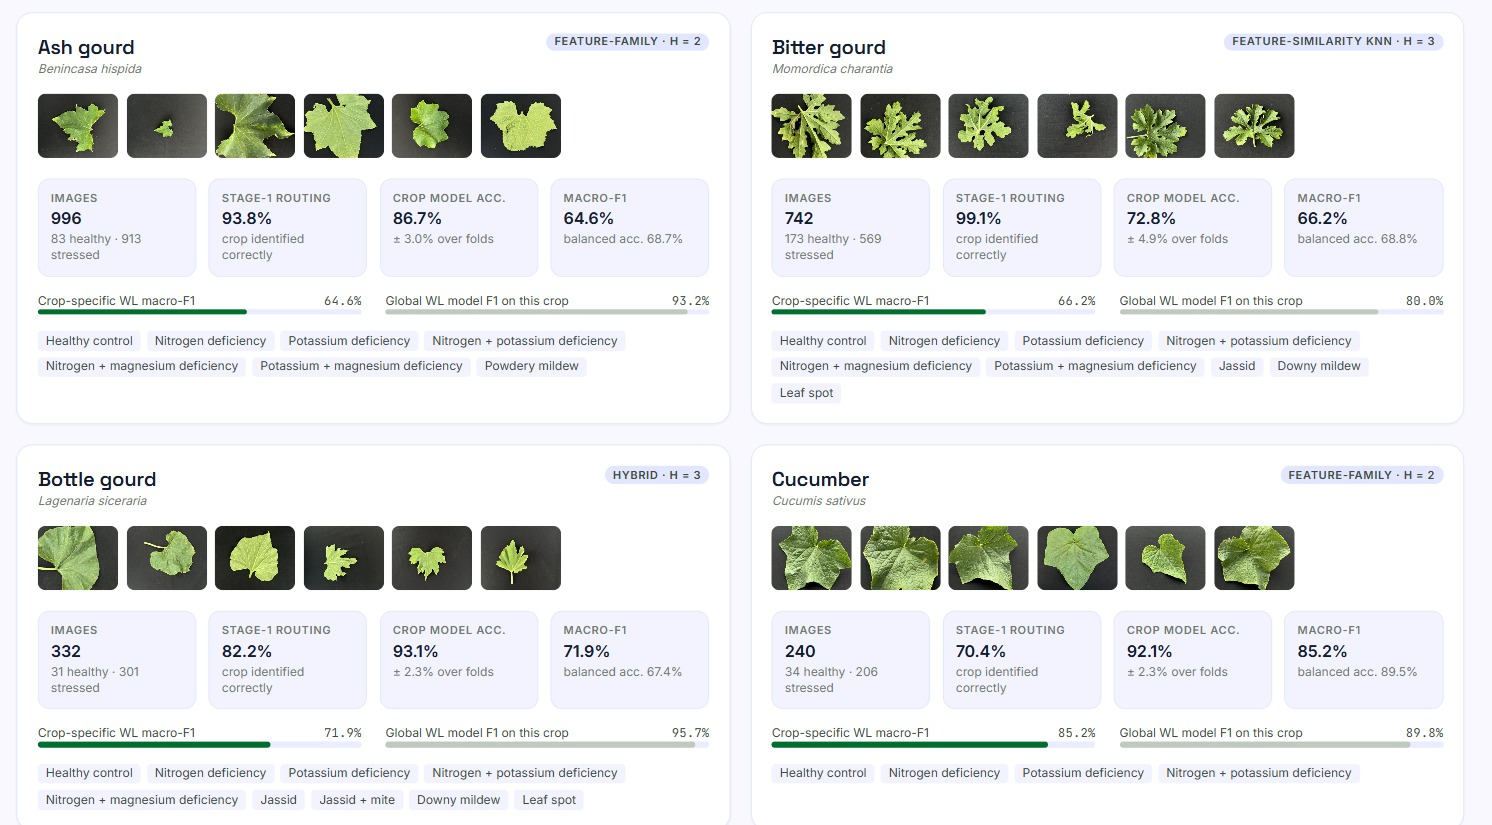
\includegraphics[width=0.92\textwidth, height=0.72\textheight, keepaspectratio]{last.jpg}\\[4pt]
    {\tiny\itshape Numbers here are for the app's per-crop models, so they differ slightly from the single-model results on the Crop Subgroup slide.}
\end{frame}

% ============================================================
% SLIDE: Limitations & Future Work
% ============================================================
\begin{frame}{Limitations \& Future Work}
    \begin{columns}[T, onlytextwidth]
        \column{0.485\textwidth}
        \begin{tikzpicture}
            \node[rectangle, draw=amritaMaroon, thick, fill=maroonSoft,
                  rounded corners=4pt, inner sep=6.5pt, text width=0.93\columnwidth, align=left] {
                {\small\bfseries\textcolor{amritaMaroon}{Limitations}}\\[3pt]
                \begin{itemize}\scriptsize
                    \setlength{\itemsep}{2pt}
                    \item \textbf{Exact condition (57 classes) not solved:} best model 0.57 macro-F1, WL 0.42. The 38 measurements are leaf \emph{averages}, so small local marks are washed out.
                    \item \textbf{Healthy leaves are hard to find} for crops with few healthy photos (bottle, ridge, ash gourd).
                    \item \textbf{Lab photos only:} one leaf on a dark background; field photos not tested.
                    \item \textbf{No severity labels} in OLID-I, so no severity grading.
                    \item \textbf{Speed:} segmenting the full 3,024\,px photo takes $\approx$1\,s.
                \end{itemize}
            };
        \end{tikzpicture}

        \column{0.485\textwidth}
        \begin{tikzpicture}
            \node[rectangle, draw=amritaMaroon, very thick, fill=amritaMaroon, text=white,
                  rounded corners=4pt, inner sep=6.5pt, text width=0.93\columnwidth, align=left] {
                {\small\bfseries Future Work}\\[3pt]
                \begin{itemize}\scriptsize
                    \setlength{\itemsep}{2pt}
                    \item \textbf{Local spot features} as extra graph nodes, to approach the 57-class task.
                    \item \textbf{Fine-tune the CNN} (currently frozen) for the strongest decision model.
                    \item \textbf{Field photos} and other datasets to test real-world use.
                    \item \textbf{Faster segmentation} on a smaller copy of the photo.
                    \item \textbf{Learned graph edges} instead of hand-chosen rules.
                \end{itemize}
            };
        \end{tikzpicture}
    \end{columns}
\end{frame}

% ============================================================
% SLIDE: Conclusion
% ============================================================
\begin{frame}{Conclusion}
    \begin{itemize}
        \setlength{\itemsep}{0.25cm}
        \item \textbf{Graph construction matters.} Linking related measurements (Hybrid / Feature-Family) beats correlation or spatial links by \textbf{7.5 points} macro-F1, and WL depth $h{=}3$ adds \textbf{9.6 points} over no graph.
        \item \textbf{WL is competitive, not the most accurate.} Macro-F1 0.706 vs 0.739 for a frozen CNN and 0.729 for tuned Extra Trees, all far above the ``always stressed'' 0.456.
        \item \textbf{WL is the most stable measurement-based model} when photos are darker, blurred, compressed or noisy.
        \item \textbf{Where WL stands out: a trustworthy second opinion.} When WL and the CNN agree (83\% of leaves) the answer is right 91\% of the time; their disagreements contain half of the CNN's mistakes, and WL explains its call in leaf terms.
    \end{itemize}

    \vspace{0.2cm}
    \centering
    \begin{tikzpicture}
        \node[rectangle, draw=amritaMaroon, very thick, fill=amritaMaroon, text=white,
              rounded corners=4pt, inner sep=7pt, text width=0.9\textwidth, align=center] {
            \small Best use: the CNN decides quickly, WL checks and explains, and the farmer sees when to double-check.
        };
    \end{tikzpicture}
\end{frame}

\section{References}
\begin{frame}[allowframebreaks]{References}
    \tiny
    \bibliographystyle{IEEEtran}
    \bibliography{ref}
\end{frame}

% ============================================================
% FRAME: Thank You
% ============================================================
\begin{frame}
    \centering
    \vspace{1.5cm}
    {\Huge \textbf{\textcolor{amritaMaroon}{Thank You}}} \\[0.8cm]
    % {\large \textbf{Questions \& Discussion}}
\end{frame}

\end{document}